\documentclass{article}

\usepackage{bm,bbm}
\usepackage{hyperref}
\usepackage{graphicx}
\usepackage{subcaption}
\usepackage{amsmath,amsthm,amsfonts,amssymb}
\usepackage[latin1, utf8]{inputenc}
\usepackage[dvipsnames,svgnames,x11names]{xcolor}
\usepackage[sort, authoryear]{natbib}
\usepackage{siunitx}
\usepackage{authblk}
\usepackage{setspace}
\usepackage{lscape}
%\usepackage[english]{babel}
\usepackage{geometry}
\geometry{left=4cm,right=4cm,top=3cm,bottom=3cm}


\title{Metabolic safety margin as an indicator of transient state of the energetic metabolism in trees}

\author[1*]{David Herrera-Ram\'irez}

\author[1]{Carlos A. Sierra}

\author[1]{Boaz Hilman}
\author[1]{Susan Trumbore}
\author[2]{Paulo Brando}

\affil[1]{Max Planck Institute for Biogeochemistry, Hans-Kn{\"o}ll-Str 10, 07745 Jena} 
\affil[2]{Yale School of the Environment} 


\begin{document}
\maketitle

\begin{abstract}
%\noindent

Non-structural carbon (NSC) reserves, especially starch, are vital for trees to survive and recover from stress. NSC dynamics leave a footprint in the age of NSC stored and allocated to respiration and growth. We propose a new measurement, the \textit{Metabolic Safety Margin} (MSM), to evaluate the metabolic state of trees and NSC turnover times by analyzing the relationship between NSC mean age and transit time.

NSC mean age is the time from carbon fixation to measurement, while NSC transit time is from carbon fixation to allocation for metabolic needs like respiration and growth. These quantities are modeled using compartmental models and a novel mathematical framework, and estimated by measuring 
$^{14}C$ in stored starch or soluble carbon and respired $CO_{2}$.

We modeled the Metabolic Safety Margin for five trees with varying NSC turnover times by adjusting NSC allocation to slow cycling storage compartments. Our models indicate that trees prioritizing storage are further from the 1:1 line and take longer to reach it under starvation. They also show a longer and slower transient response of the MSM to reduced carbon income.

We estimated the age of soluble carbon and respired $CO_{2}$ in the stem wood, branches and roots of trees in the amazon with contrasting storage strategies and trees in the the Swiss Alps using $^{14}C$. Results suggest that MSM in sipecies with high priotity to storage is further from the 1:1 line. Additionally, MSM in roots and stem wood may provide more long term metabolic informatio than MSM in branches, probably because their slower NSC turnovertimes. 

The Metabolic Safety Margin helps evaluate the metabolic state of mature trees and their resilience to environmental stress, improving estimates of tree vulnerabilities to climate change.

\end{abstract}



\section{Introduction}

Trees are long-lived organisms that face and survive multiple and frequent stressors and disturbances along their life-span. 
Global change is increasing the frequency and severity of stress and disturbances by incresing air temperature, vapor pressure deficit (VPD), and shifiting precitipation regimes, affecting trees all over the world. 
%These changes interact with global climatic patterns and increse the frequency and severity of multiple disturbances that affect tree survival, growth and reproduction.  
The combination of these factors is expected to caused changes in forest demographics with severe consequences for the global carbon cycle and for the climatic crises we now face. 
Understanding the vulnerability of trees and forests to these new set of conditions and their survival and recover is paramount for us to predict changes in forest composition and functionality facing new global environmental conditions. 

Tree's investment into carbon reserves help them to survie and recover from multiple disturbances or stresful changes in environmetnal conditions.
Carbon reserves in the form of nonstrucural carbon (NSC) are mainly solble surgas, starch and lipids. 
These reserves can be short-term -cycled very fast with a high turnover- or long-term -cycled slower with lower turnover- depending on the organ they are stored and the tree species.
Tree species differe in their carbon allocation strategies and some may priotitize allocation to NSC long-term storage over other allocation alternatives such as growth.
Thus, trees storing long-term NSC may have very old reserves that, if accessible, can buffer metabolism at multiannal or multidecadal time scales, playing a fundametal role in long term tree survival and recovery.  

%These reserves may serve as a energy source when trees face negative carbon balances, which enables trees resilience to compounding disturbances and stressful conditions such as higher temperatures and higher VPD.
%Some trees cycle these reserved rapidly, while some other trees form longer-term carbon reserves that can be stored for several decades in organs such as stem-wood and coarse roots,  and can be access after a catarstrophic disturbance to recover from damage. 


Under a positive carbon balance, trees' metabolism is sustained by recent NSC. 
However, when trees are in a carbon deficit, they access their reserves to sustain metabolism.
In these conditions, the carbon allocated to metabolism starts reflecting the contribution of old reserves, becoming progressively older. %while the contribution of older reserves to respiration and growth increases. 
When trees recover or adapt NSC reserves replenish with new NSC, and allocation to metbaolism comes back to rely on younger NSC. %As carbon fluxes to growth may decrease carbon allocater of older reserves would be reflected in older respired $CO_{2}$. 
Thus, the interpla between multiple disturbances alogn trees' life span and trees' carbon metabolism would leave footprints in the composition of ages of the NSC reserves and the NSC being allocated to metabolism.
% that could be reflected in the relationship between the age of the respired $CO_{2}$ and the age of the stored NSC. 


We lack a mechanistic undestanding of how strees and disturbanes impact the use of carbon servers and the trees carbon fluxes that would determine the age composition of the carbon reserves and the age of the carbon allocated to metabolism. 
Despite its importance, there are few studies that characterize the age and turnover time of NSC in mature trees under stress or when facing multiple disturbances. 
This is because the lack of technics that allow us to estimate NSC turnover times in mature trees, and because keeping track of changes in trees' carbon fluxes over time is expensive and time consuming. 
Evaluating the footprints that multiple disturbances may leave on the NSC age composition would be a feasible alternative to investigate how stress impact the use and recovery of NSC reserves.
This would help us to estimate how much a tree has been metabolically affected by past disturbances and how vulnerable they may be to the upcoming ones. 
%This information would help us to estimate tree survival an recovery from multiple disturbances and from changes in growing conditions due to climate change. 
%Understandind how this compositional changes would happen over the most important forests in the world is essential to better estimate biospheric carbon fluxes in the 

%Tree survival and recover from compounding disturbances or permanent changes in growing conditions would depend on how the balance between carbon sources and sinks would adapt under the new conditions. 
%Tree mortality, in most of the cases, is not the cause of one specific disturabance, but the result of coumpound disturbances happening over time that affects tree metabolism. 
%Mortality during drought, for instances will not only depend on the hydraulic failure (which may be the cause) but will be also strongly influence by the previous disturbances (physical damange, deseases, pests) that a tree may have experienced over time and that would have affected the metabolic status of that individual tree. 
%Keeping track of this disturbances is difficult, but they leave a fingerprint in the carbon metabolic status of the tree, which can be assessed to estimate the vulnerability of trees to die under new upcoming disturbances or new growing conditions. 


Here we want to present a new metric to evaluate te status of carbon metabolism of trees and their vulnerability to future stressful condition.
The metabolic safty marging, as we call it, is the relationship between the age of the NSC allocated to metabolism and the age of the store NSC in trees (Fig. \ref{fig:NCSage_CO2age}).
This metric serves as a proxy to understand the interplay between trees carbon balance and changes in environmental conditions. 
We hypothesize that this relationship integrates the metabolic history of an adutl tree over the recent years and would indicate how much a tree has been affected by past multiple perturbations and how vulnerable it will be to future extreme events or changes in growing conditions. 




%Justify what is the problem that the new Idea is going to solve 
%\subsection{Problen}
%
%main question: 
%
%start with why measuring metabolic status is important. tree mortality is a metabolic problem in many intances: after drought, after damages... etc. 
%How do we know the metabolic status of trees? 
%
%mortality not only depends on one specify disturbance but on the compound disturbances which affects metabolism. Mortality during drought events for instances will depend not ontly on the hydraulic traits but will also be strongly influences by previous crown disturbances (physical damage, deseases), and this my be for other events. Reconstructing previous disturbances is hard, but each disturbance leaves a footprint in the carbon metabolis. So this footpring is observed in the relationship of the age of the respires carbon with the age of the stored carbon.
%
%how can we reliably assess the metabolic status of the carbon reserves of individual trees in order to predict how capable is a tree to survive compounding perturbances and to recover from them?  How the ration between the age of the respired CO2 and the age of the stored NSC can give works as an integrator of the metabolic history of a tree which at the end is  the fitness optimization for survival and therefore can tell us about how affected has been the tree by the past perturbations and how vulnerable is the tree to future perturbations. 
%
%%Can this individual assessment of trees metabolic status be upscaled to the forest scale? 
%
%Tree survival and recovery from many compounding disturbances depend on the balance between sources and sinks. 
%This balance is buffered by NSC. 
%Therefore tree survival and recovery from stress is influenced by the reserves status and NSC metabolism. 
%
%It is challenging to measure the carbon reserve status and NSC dynamics in mature trees, and this brings a lot of uncertainties to the understanding of the influence of NSC on tree survival and recovery. 
%NSC fluxes as many physiological fluxes can be very plastic in their response to environmental changes and can vary a lot depending on the conditions that a tree experience. 
%Nevertheless, trees vulnerability to stress also depends on the past compounding perturbances a tree has experiences before, which may not be directly reflected in the NSC fluxes measured under some specific conditions (at a given point in time). 
%To assess trees vulnerability to some stressors it is necessary to understand how trees have balanced their sources and sinks activity over time.  
%For that it is necessary to measure repeatedly NSC fluxes, as well as carbon source and sink fluxes.
%This is challenging, expensive, not very precise and very time consuming.  
%
%The relationship between transit time and the mean age of the stored NSC can work as an integrator of the influence of the current and past stressful conditions on trees metabolism and the history of the balance between sources and sinks. %(can this be analyzed with the optimality theory??). 
%Therefore, these traits can give us better information on the metabolic status of trees respect to their carbon reserves and the potential of trees to survive and recover from compounding perturbations (INCLUDE HERE A CONCEPTUAL FIGURE TO EXPLAIN). 


%Include the idea from zuleta: mortality not only depends on one specify disturbance but on the compound disturbances which affects metabolism. Mortality during drought events for instances will depend not ontly on the hydraulic traits but will also be strongly influences by previous crown disturbances (physical damage, deseases), and this my be for other events. Reconstructing previous disturbances is hard, but each disturbance leaves a footprint in the carbon metabolis. So this footpring is observed in the relationship of the age of the respires carbon with the age of the stored carbon. 


%
%Make the problem about vulnerability or forest health in general?
%
%How to evaluate trees health in a forest? how to tell the stress history that trees has experienced. tress are not only impacted by inmediate perturbation but also by perturbations that they have standed before which might have debilitated them and made them more vulnerable. 
%vulnerability is not only the capacity of one single event to kill a tree, but also the state of the tree given the past event they have withstanded. 
%
%NSC dynamics and many physiological traits are very sensitive to transient conditions in the environment and can adapt very fast to environmental changes, nevertheless the impact of stress on trees and forest is long-lasting and can bring trees to death after many years of ocurrence, then how do we actually tell the impact that this stress changes have had over trees metabolism. 
%
%The transit time and mean age of the NSC in trees can work as an integrator of not only the stress conditions that trees are experience but also they hold the record of the impacts of the past stressful conditions and can give a blink on how healthy (or how much pressure) is the carbon metabolism of trees in order to predict mortality and vulnerability. 
%
%
%tree health and ecosystem health are entangled. To assess ecosystem health we need to understand how healthy are the trees that constitute those ecosystems. 
%
%Tree survival depends on the balance between sources and sinks, which are actually buffered by NSC. 
%
%Nevertheless, it is difficult to measure NSC dynamics and other carbon sources and sink dynamics (e.g. photosynthesis and respiration) over time and at different tree organs.
%growth is only measured mainly at the stem wood. 
%
%It is also difficult and practically impossible to differenciate between storage and active pool in the more than one model of storage pools...
%So it is difficult to determine how much of the stored NSC is actually or would actually be used for trees to cover metabolism when balancing carbon sources and sinks. 
%
%scaling up NSC concentration measurements to tree level and ecosystem level is charged with tons of uncertainties that impair using this measurements to predict tree mortality or recovery. 
%
%Therefore it has been difficult to link carbon dynamics in trees with trees ability to survive and recover from stress. 


\section{Metabolic stafety margin: a new metric to evaluate the metabolic status of mature trees}

Carbon reserves (NSC) are thought to be rapidly cycled in trees. 
Nevertheless, turnover times of NSC can vary from organ to organ and from species to species.
For instance, they are cycled at a daily basis in leaves, but they may be multiannual in the long term reserve pools such as the stemwood. 
The time that they can be store in the stemwood highly depends on the sepecies and the wood anatomy. 
NSC turnover time also depends on the pool size and the carbon fluxes towards metabolic needs such as respiration and growth.
Besides, this NSC turnover time would vary as trees regulate their carbon fluxes as function of environmental conditions. 
The strategy for the storage and use of long term reserves affects trees carbon fluxes and metabolism, which relfects on the capacity of trees tu survive certain disturbaces or stresful conditions and recover. 

Estimates of the age of the NSC stored in trees could serve as a proxy for the NSC turnover time, if trees are in steady state. 
Age of the NSC can be defined as the time between the carbon fixation by fotosynthesis until the time of observation. 
Large carbon allocation to NSC reserves and low carbon allocation to growth, respiration and reproductions would result in low turnover times.
The lower the NSC turnover time the older NSC would become in the reserve pools.
%Some trees can store NSC for decades in these organs. 
Nevertheless, NSC turnover time have high variability.
There are, in nature, trees with very fast NSC turnover which results in very young stored NSC and trees with reserves that have been stored for decades. 
NSC turnover time may also vary algon trees life span or may change in response to environmental stressors, although changes in NSC turnovertime may imply changes in the carbon allcation strategy. 
Some of these stored reserves, old or young, remain available over time to support metabolism and growth when trees face stressful conditions or have to recover from disturbances, playing a fundmental role in trees resilience to environmetal changes. 

As trees are not usually in steady state, and NSC pool size and carbon fluxes changes with envoironmental conditions, the observed age of the NSC alone may not be a good proxy of the NSC turnover time. 
%Trees are subjected to frequent and compound disturbances which have an impact in the carbon balance and in the metabolic response of trees to the environment. 
Furthermore, NSC ages are not homogeneusly distributed in trees or tree organs.
The distribution of ages may depend on the mixing rates between old stored NSC and newly assimilated carbon, which may be determined by trees life history traits. 
Fluctuations of the carbon balace and the carbon mixing rates influence the age composition of the NSC reserves and create transient responses on the NSC ages that are not the reflection of changes in the NSC turnover time. 

These differences in the NSC age distributions and fluctuations in the carbon balance in trees make the age of the allocated carbon to metabolism differ from the age of the NSC stored in the reserve pools.
NSC transit time is the age of the carbon since it enters the tree until it is allocated to other carbon sinks rather than NSC (e.g. respiration, growth, reproduction or exudates).  
Then, here we can regard the age of the NSC allocated to metabolism and the NSC transit time. 
Thus, for mature trees that face multiple disturbaces we would expect that the average mean age of the NSC in the a tree is different to the average NSC mean transit time. 
The relationship between these two metrics and its changes over time can give us insights about the metabolic state of trees and their response to multiple disturbances. 

Trees under a positive carbon balance would usually allocate a larger propotion of young carbon to metabolism.
Usually carbon allocated to respiration and growth in healthy trees range from 1 to 5 years of age, on average.
When trees are under a negative carbon balance, they access carbon reserves to sutain their metabolism and survive. 
As disturbances or stress progress,  the contribution of old reserves to metabolic functions progresively increases. 
This contribution of old reserves to trees metabolism would be reflected in the NSC transit time.
As stress progress in trees, NSC transit time becomes progresively older as much as the age composition of the available reserves allows it.
This progression help us understanding how fast trees can access their reserves and for how long carbon reserves in trees reamain availabe, helping us to better understand transient responses of NSC ages in trees in response to environmental changes.  

Then, the relationship between the NSC mean transit time and the NSC mean age at a given time may help us to estimate how much of the long term reserves are contributing to trees metabolism, relative to the NSC turnover times of individual trees. 
For instances, when trees cycle NSC very fast and do not store NSC for long periods of time, this ratio would always be very close to 1, meaning that due to the fast NSC turnover time trees reserves would not last very long under extreme stressful conditions that result in a negative carbon balance. 

When trees have slower NSC turnover time, they would have older stored NSC. 
In healthy conditions, these trees may have very young transit times and old reserves, making the relationship between the NSC mean transit time and NSC mean age smaller than one. 
Nevertheless, under stressful conditions trees may start accessing these reserves and the transit time would become older leading this relationshipt closer to 1. 
This transient response show us how much trees are relying on the old storage to maintain their metabolic functions. 
When the relationship between the transit time and the age of the stored NSC gets closer to 1, it may indicate an exahustion of carbon reserves.
This can happen because a transient change in the composition of NSC age or because a change in the NSC transit time, or both.
These changes may indicate a more vulnerable state of trees to upcoming disturbances. 

We propose here using this relationship between the NSC mean transit time and NSC mean age and its relative distance to the 1:1 line as a metric to evaluate the trees vulnerability to stress and disturbances, and their capacity to recover (Fig. \ref{fig:NCSage_CO2age}). We named it ``metabolic safety margin" and would serve as a proxy of the transient change in NSC age composition or in NSC turnover time that trees may experience in a given moment, and would help us evaluate the metabolic health of adult trees. 



%
%The relationship between the age and the transit time of NSC in a tree system (Fig. \ref{fig:NCSage_CO2age}) give us integrated information about the past and the present carbon metabolic status  that reflects the balance between carbon sources and sinks that trees have experienced over time, as well as the turnover time of the NSC reserves under transient conditions. 
%
%This relationship would show us in a single time point whereas trees have managed, during their lives, to put apart some reserves for several years to face future stressful conditions and how much these reserves are contributing to sustain the current metabolism. 
%Basically, the idea is to evaluate how close to 1 the relationship between the age and the transit time of NSC is for a given tree organ. 
%
%
%Healthy trees generaly respire young carbohidrates. 
%Trees may store carbohydrates for short periods or long periods of time. 
%This may be related to the age of the tree and the life history of a tree. 
%For instance young trees can only have young NSC reserves, but trees with a fast NSC turnover time would also have younger reserves respect to their age. 
%Old trees may have store long term reserves of NSC and wouldhave old age of stored NSC. 
%If these old trees are healthy they would still be respiring young CO2 in comparison to the stored NSC. 
%The closer to 1 the relationship between the age of the respired CO2 (NSC transit time) and the age of the NSC would indicate for how long trees have kept they NSC storage and how much it has been used due to the incidence of past stressful conditions. 
%
%
%BETTER TO STICK WITH CHANGES IN THE AGE COMPOSITION INSTEAD OF TALKING ABOUT TURNOVER TIME? 
%The closer to 1 this relationship is will also indicate the transient response in the use of carbon reserves for these trees. % in our models, as they are linear time-dependent, the turnover time remains constant in each time step (because the cycling rates do not change), there is always the same proportion of C leaving the system relative to the amount of C staying in the system.
%This will also indicate an appearent increase in the turnover time causes by the stressed applied to the system??. %we can say this in terms of how trees would behave. 
%when this relationship gets closer to 1 it may indicate a faster transient turnover of NSC in the trees, even if NSC ages and the age of the respired CO2 are old (maybe we shouls show this with equations).
%If we consider carbon turnover time as the relationship between the C flux out of the system and the carbon stock in the system, fast turnover, indicated by low values may indicate that the system replaces the cabon very fast, and the age of the flux out and the stock carbon would be both very young and therefore their relationship would be close to one. 
%When a tree has lower fluxes of NSC out in relation to the store NSC the turnover time get slower, indicadet by bigger values, and therefore the age of the stock C gets older over time, althow the ager of the flux out may stay young due to the system dynamics and structure. 
%Turnover time of the NSC in trees may not be constant over time, basically because carbon fluxes are sensitive to environmental conditions, so they are transient turnover times. 
%An increase in the transient turnover time of the NSC in a tree will indicate a reduction of the carbon stock or and increase in the flux out. 
%This will result in an increase of the age of the socked carbon and an increase in the age of the flux out. 
%Wehn this relationship gets closer to 1, it will indicate that the sotred NSC is getting lost at a faster rate than it is replaced by young NSC and therefore the age distribution of the carbon flux out is getting closer to the age distribution of the remaining stored NSC. 
%
%A fast turnover time of NSC will indicate may make trees more vulnerable to uncertain future conditions, and can reduce their resilience. 
%therefore a relationship between the mear age and the transit time of the NSC closer to on may indecate as well that trees have expirienced compounding distrubances that do not allow them to recover the NSC stocks and cycle them at slower turnover rates and therefore they may be more vulnerable and less resilient to future disturbances of more difficult growing conditions.  

%Measuring transient turnover times is expensive a time consuming.
%
%
%
%If trees have experience several compounding and frequent disturbances that have maintain a negative carbon balance over time, the relationship between the mean age and the transit time of the NSC in trees would be closer to the 1:1 line, and trees may be more vulnerable to die if they experience new disturbances. 
%If trees have had positive carbon balance over time, and they prioritise reserves over growth and reproduction, they would store NSC for longer time, making the stored reserves older and older over time while relying mainly in newly fixed carbon to sustain metabolism. 
%Then, the relationship between the age and the transit time of NSC would be farther away from the 1:1 line and these trees would have larger capability to stand a stressful condition and recover from them. 


 \begin{figure}[h] %  figure placement: here, top, bottom, or page
   \centering
   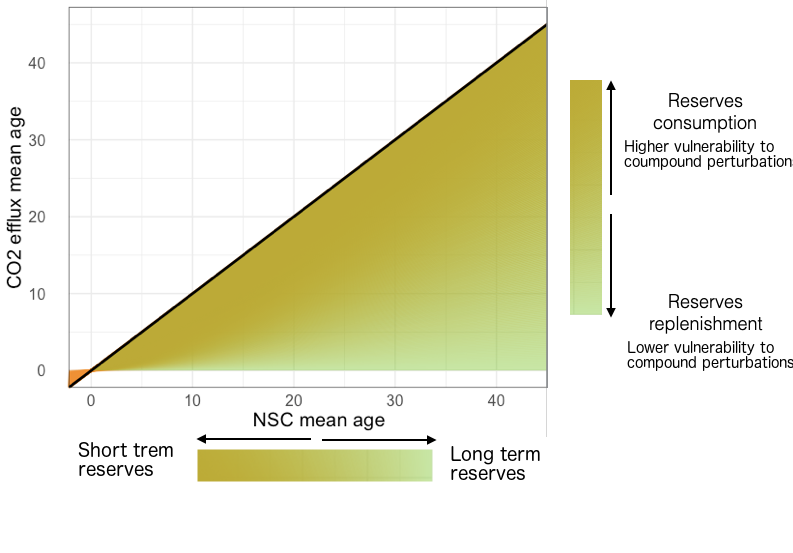
\includegraphics[width=5in]{NCSage_CO2age.png} 
   \caption{Theoretical relationship between the NSC mean age and the NSC transit time. Darker colors show a closer proximity to the 1:1 line which indicates a faster NSC turnover time}
   \label{fig:NCSage_CO2age}
\end{figure}


%explain better how different trees under different conditions would be  in the data space, and how it would affect our interpretation of results. be clear about the balance between sources and sinks and not about specific conditions (the main thing is to integrate over the impact of compounding disturbances) 
 

\section{Estimates of the metabolic safety margin}

Estimting NSC mean age and NSC mean transit time for entire mature trees is challenging, but we can consider good proxies to rely on for estimating and measuring these two quantities. 
%Interest on the age of trees' NSC have increased over the recent years, although studies remain scarce. 
%For instance, Age of the store and available NSC (soluble carbon and starch) have been estimated and reported for some tree tissues using $^{14}C$. 
%The age of the NSC allocated to respiration and growth have also been documented in girdling experiments and in trees recovering from strong disturbaces, to ilustrate how different tree species access their reserves to revocer. 
For insntace,  $^{14}C$ measurements in the soluble carbon, starch, respired $CO_{2}$, and new wood formed after cathastrophic events have been used to estimate NSC ages and allocation of carbon to metabolism during stress. 
Alternative, these quantities have also been modelled. 
Models allow us to estimate the NSC mean ages and transit time in specific organs and in the entire tree.
They also allow us to estimate the distribution of NSC ages and transit time and their variability between tree species and tree organs. 
In the following sections we will ilustrate how both thecniques help us estimating and understanding the metabolic safety margins. 

\subsection {Modelling approach}

Metzler et al 2018 have developed an inovative mathematical framework to estimate mean ages and mean transit time for compartimental systems.
This framework have been recently used in several studies to estimate differences in age composition of NSC in trees with different storage strategies or growing at different environmental conditions. 
One way to explain carbon alocation is dividing NSC in several compartmets in trees.
Carbon gets into the system as sugars fixed from photosynthes that are distributed to several compartmentes such as leaves, stem and roots.
Then, in each organ it may be allocated to NSC reserves, respiration, biomass, reproduction, defense compounds or exudates.
We can use this conceptual compartimentalization of NSC allocation to estiamte the NSC mean ages and transit times  for each defined compartment and for the whole tree using the matematical framework proposed by Metzler et al 2018. 

As an example, to estimate the mean age and mean transit time of NSC of trees with different allocation strategies and its changes following stressful conditions or disturbances, we used the NSC compartimental model adapted from Herrera-Ramirez et al 2020 and Klein and Hoch 2014 (Fig. \ref{fig:comp_model}). 
This model considers leaves, stems and roots as organ comprtments and in each of these organs it considers two NSC compartments: stored NSC (slow cycled) and active NSC (fast cycled) (Table \ref{table:name_compartments}).
For simplicity, only allocation to growth and respiration was considered as the ouflux of carbon from each compartment/organ (Fig. \ref{fig:comp_model}.
With these models we wanted to explore the differences in the metabolic safety margin of trees with different storage strategies and different NSC turnover times and describe their rsponse to stressful conditions such as starvation or photosynthetic reduction. 

\begin{figure}[h] %  figure placement: here, top, bottom, or page
   \centering
   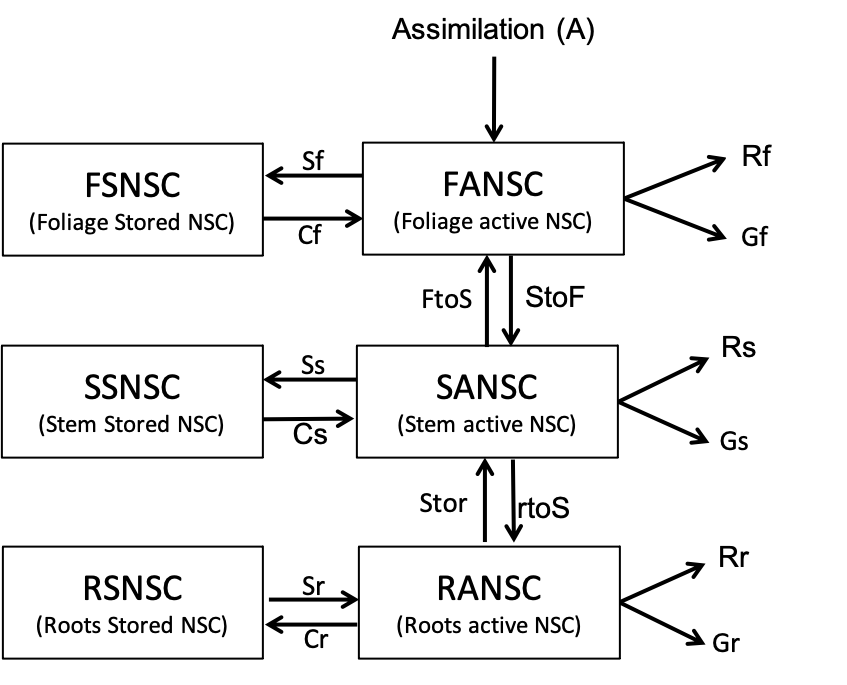
\includegraphics[width=3in]{Fig_comp_model.png} 
   \caption{NSC allocation compartimental model. This model considers three organs foliage, stem and roots. In each orgar there are two NSC compartments an Active fast cycling compartment and a storage slow cycling compartment. Compartments are indicated by boxes, while fluxes out and into compartments are indicated by arrows. Abreviation names are explained in Table \ref{table:name_compartments} and  Table \ref{table:parameters}}
   \label{fig:comp_model}
\end{figure}  


\begin{table}[ht]
\caption{Compartments description for the model structure proposed in Fig. \ref{fig:comp_model}} % title of Table
\centering % used for centering table
\begin{tabular}{cc}
\hline \hline
Abbreviation  & Name  \\
\hline
E & Transient Carbon Pool  \\
FANSC & Foliage Active Non Structural Carbon  \\
FSNSC & Foliage Stored Non Structural Carbon  \\
SANSC & Stem Active Non Structural Carbon  \\
SSNSC & Stem stored Non Structural Carbon  \\
RANSC & Fine Root Active Non Structural Carbon  \\
RSNSC & Fine Root Stored Non Structural Carbon  \\
\hline
\end{tabular}
\label{table:name_compartments} % is used to refer this table in the text
\end{table}

We parametrized these models to simulate trees with different storage strategies Table. \ref{table:parameters}. 
Parameters in these models represent the annual fraction of carbon leaving each pool, which can be estimated as the flux of carbon out of the pool divided by the size of the pool. 
We simulated a tree with a very high NSC turnover time (1 year) where all parameters have a value of 1. 
Then we simulated trees with slower NSC turnover time by changing the parameters of allocation to storage to respecto of the model with NSC turnover time of 1 (Table. \ref{table:parameters}). 
Thus we generated four more modeles with varying NSC turnover time as follow: 
1) allocation to stem storage; we increased the allocation to storage in the stem wood by a factor of 60; 
2) high allocation to stem storage;  we increased the allocation to storage in the stem wood by a fator of 120,
3) high allocation to root storage;  we increased allocation to storage in the stem wood by a factor of 60 and we the allocation to storage in the roots by a factor of 120;
and 4) low allocation to stem storage; we increased the allocation to storage in the stem wood by a factor of 30.  
These modifications allow us to evaluate the mean age and mean transit time of trees with different storage strtegies and different NSC turnover times at steady state. 

\begin{landscape}
\begin{table}[ht]
\caption{Annual rates of carbon cycling  $(year^{-1})$ and other parameters for each species from the models in Figs \ref{fig:comp_model}. Pool name abbreviations are defined in the table \ref{table:name_compartments}} % title of Table
\centering % used for centering table
\resizebox{\linewidth}{!}{
\begin{tabular}{ccccccc}
\hline\hline 
Abbreviation & Name & 1 year turnover time & stemstorage & High stem-storage & High root storage & low stem-storage \\[0.5ex]
\hline
A & Assimilation  & 230000 & 230000 & 230000 & 230000 & 230000 \\
Rf & Respiration foliage & 1 & 1 & 1 & 1 & 1 \\
Rs & Respiration stem & 1 & 1  & 1 & 1 & 1 \\
Rr & Respiration roots  & 1 & 1 & 1  & 1 & 1 \\
Gf & Growth foliage  & 1 & 1 & 1 & 1 & 1 \\
Gs & Growth stem  & 1 & 1 & 1 & 1 & 1 \\
Gr & Growth roots  & 1 & 1 & 1 & 1 & 1 \\
Sf & Allocation to storage in foliage (FSNSC) & 1 & 1 & 1 & 1 & 1 \\
Ss & Allocation to storage in stem (SSNSC) & 1 & 60 & 120 & 60 & 30 \\
Sr & Allocation to storage in roots (RSNSC) & 1 & 1 & 1 & 120 & 1 \\
Cf & Remobilization from storage in foliage (FSNSC) & 1 & 1 & 1 & 1 & 1 \\
Cs & Remobilization from storage in stem (SSNSC)  & 1 & 1 & 1 & 1 & 1 \\
Cr & Remobilization from storage in roots (RSNSC)  & 1 & 1  & 1 & 1 & 1\\
FtoS & Allocation from foliage to stem & 1 &1 & 1 & 1 & 1\\
StoF & Allocation from stem to foliage & 1 & 1 & 1 & 1 & 1\\
Stor & Allocation from stem to roots & 1 & 1 & 1 & 1 & 1\\
rtoS & Allocation from roots to stem & 1 & 1 & 1 & 1 & 1\\
\hline
\end{tabular}
}
\label{table:parameters} % is used to refer this table in the text
\end{table}
\end{landscape}



We estimated NSC mean age and NSC men transit time at steady state, for each of the 6 modeled tree types (Fig. \ref{fig:msm_steady}).
These points represent the metabolic safety marging of trees whith contrasting storage strategies at steady state.  
%These estimates are the starting point of each trayectory showed in Fig. \ref{fig:starvation}. 
%Points indicates the metabolic safety margin at each time point was time passes and the starvation intensify for each simulated tree.
Here we could observed that lower NSC turnover times (represented by higher allocation of carbon to storage in wood and roots, red and blue points in Fig. \ref{fig:msm_steady}) resulted in older NSC mean age and younger NSC mean transit time relative to storage than trees with faster turnover time (brown and black points, Fig. \ref{fig:msm_steady}). 
Thus, the closer the relationship between the NSC mean age and the NSC mean transit time is to the 1:1 line the faster the turnover time of NSC. 


 \begin{figure}[h] %  figure placement: here, top, bottom, or page
   \centering
   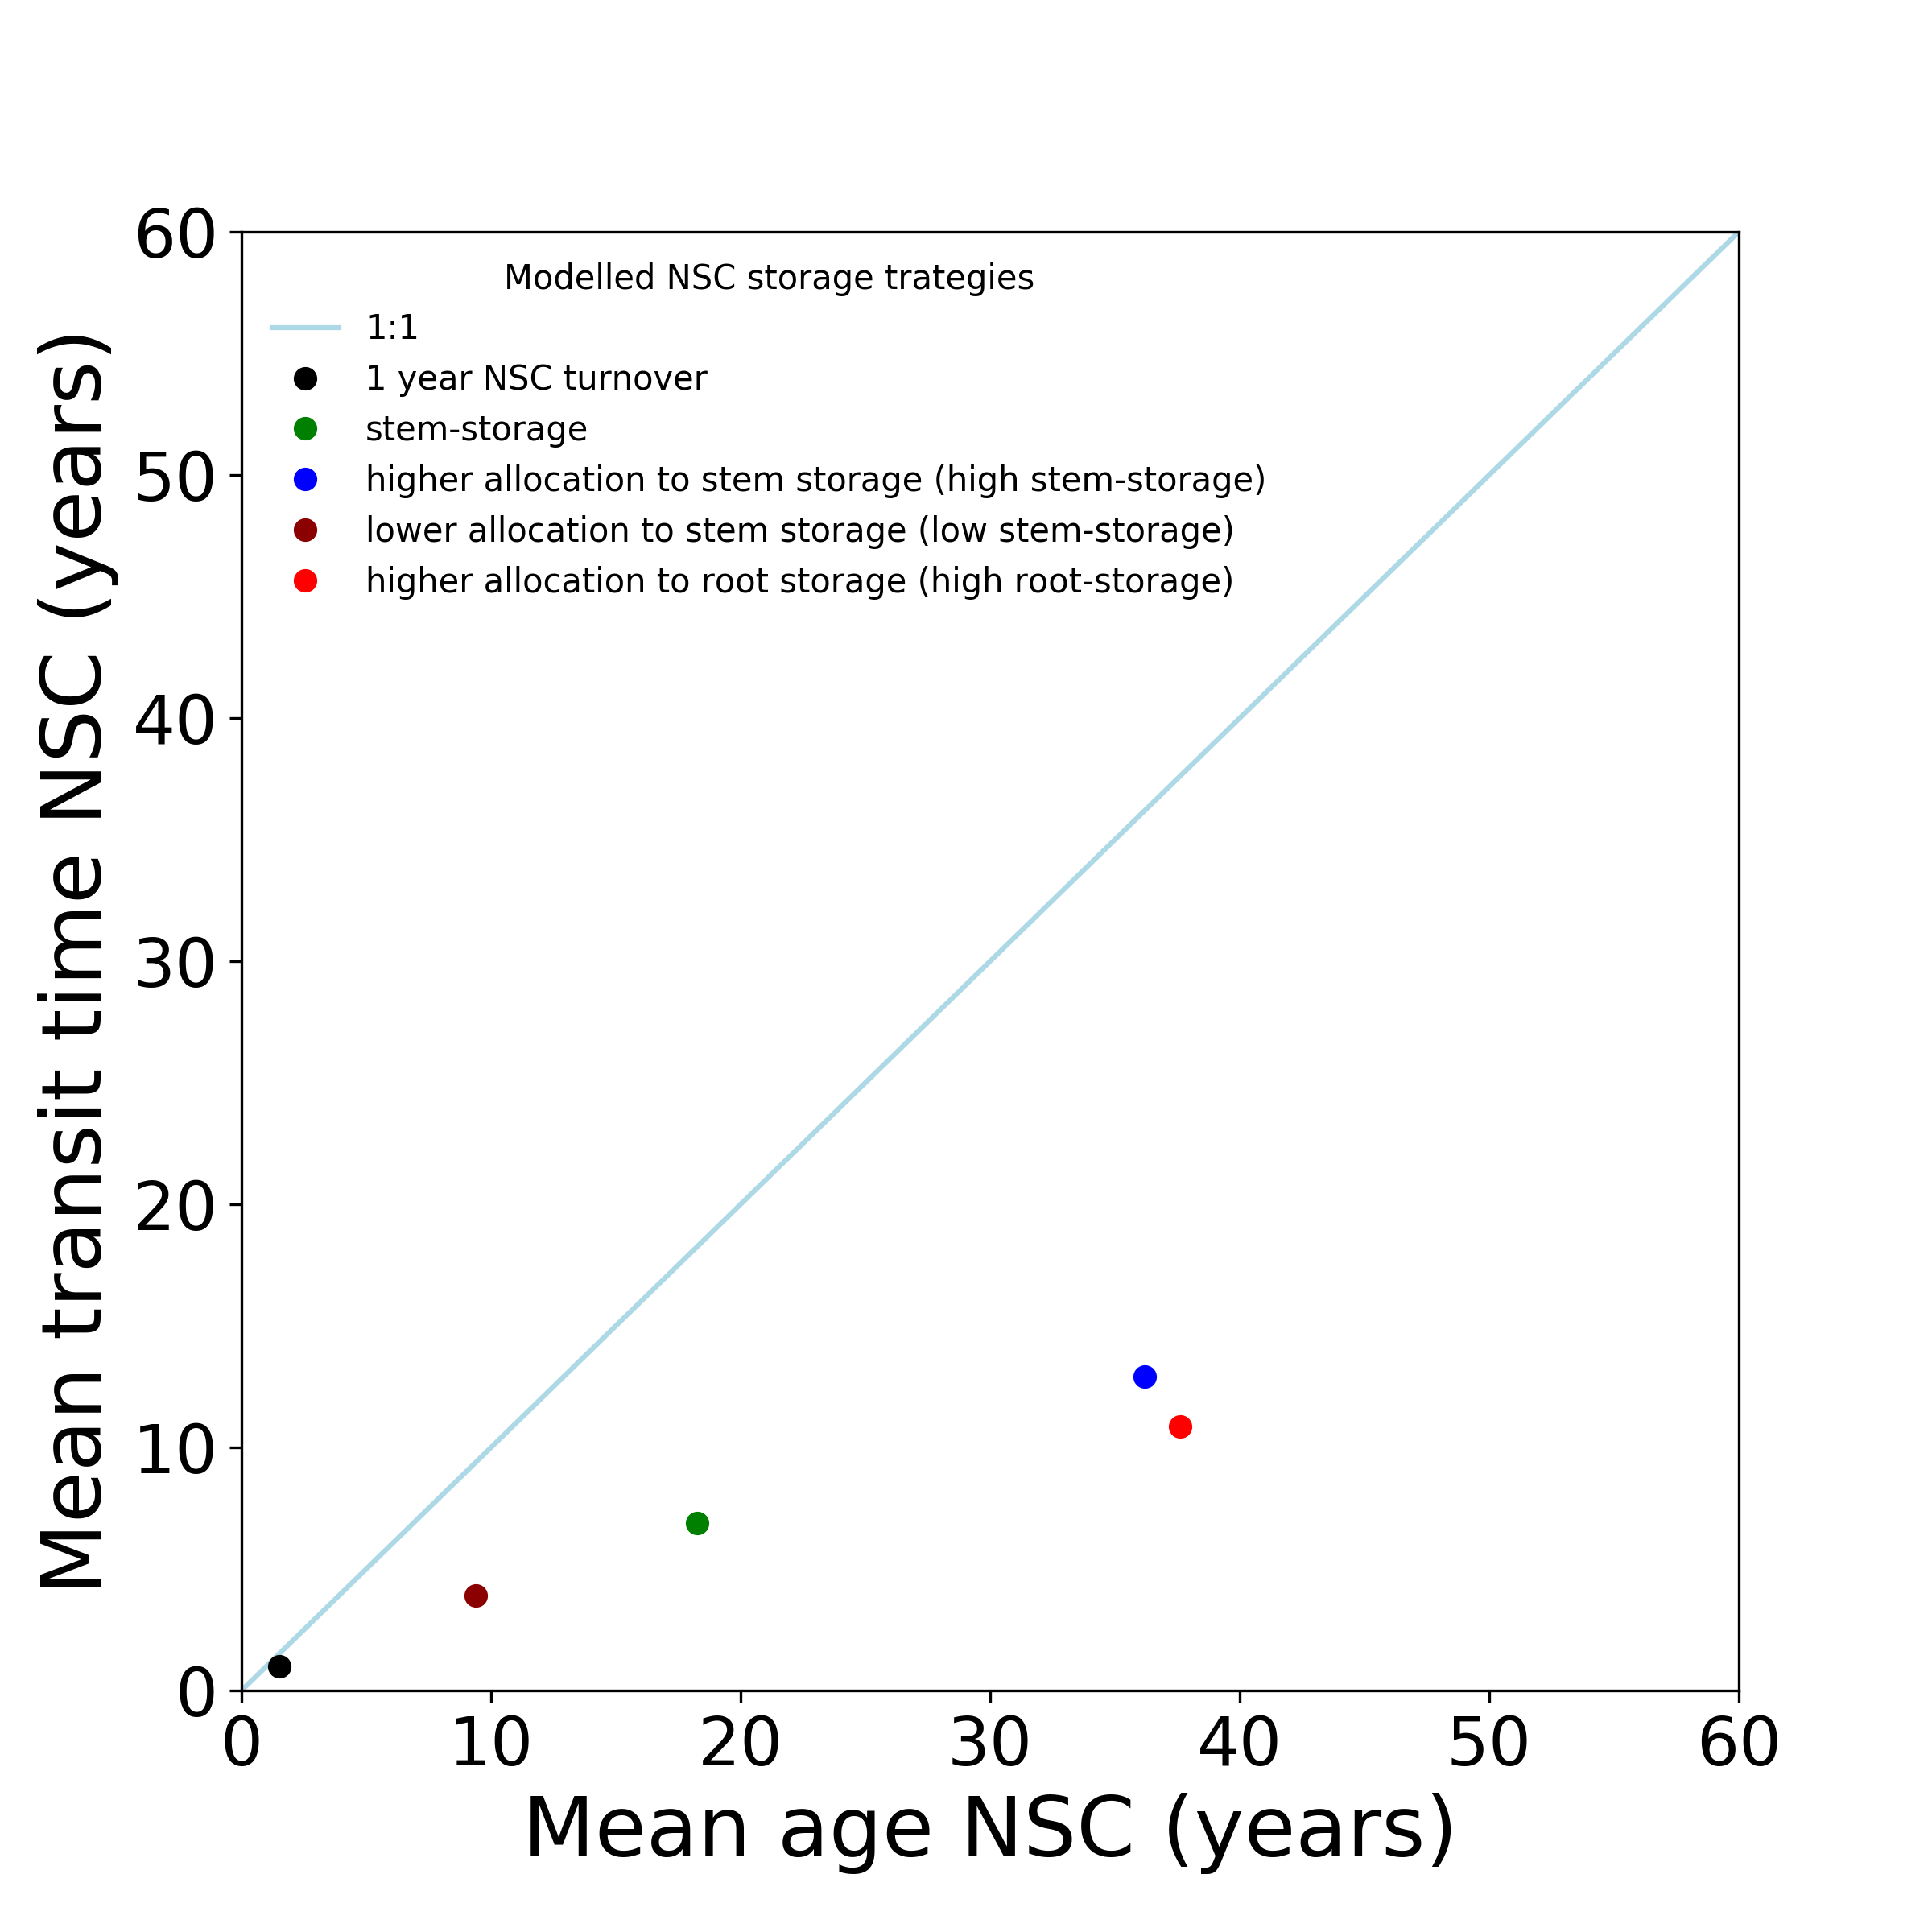
\includegraphics[width=5in]{metabolic_safety_steady_state.png} 
   \caption{Metabolic safety margin simultated for 5 trees with different NSC turnover times using the model structure presented in Fig. \ref{fig:comp_model} and the parameters described in Tale \ref{table:parameters} to generate each of the point shown in the model}
   \label{fig:msm_steady}
\end{figure}

We estimated the trajectories of the metabolic safety margin when trees with different storage strategies face starvation. 
We observed that all models shows a trajectory towards the 1:1 line while the system was getting depleted of carbon (Fig. \ref{fig:comp_model}). 
These trajectories aproach differentially to the 1:1 line depending on the NSC allocation strategy. 
For instance, high priority to storage resulted in slower approach to the 1:1 line, with a longer pathway for the larger allocation of NSC to roots (red line) than the larger allocation to stem storage (blue line) (Fig. \ref{fig:comp_model}).
Meanwhile, lower priority to NSC storage and faster NSC turnover resulted in a fast approach to the 1:1 line (green, brown and black line Fig. \ref{fig:comp_model}). 
This progresive approach of each line to the 1:1 line refelcts the incremental contribution of the stored reserves to respiration and growth.% if carbon outflux ot the NSC root storge or NSC stem storage do not change, meaning a linear not time dependent compartmental model.

These models are linear and not time dependent, therefore NSC turnover time do not change during the simulated starvation, and the estimated changes in the NSC mean age and transit time are a transient response of the age composition of the stored NSC to the simulation of starvation.
These changes in the metabolic safety margin give us insights about the ability of trees with different storage strategies to use the stored carbon when facing starving conditions and the amount of time they would take to exhaust NSC reserves, assuming no changes in the NSC turnover times. 
Changes in the NSC turnover time can happen wen trees respond to environmental conditions, reflecting a change in the tree's carbon allocation strategy.
Changes in the NSC turnover time would result in changes in the metabolic safety margin line accelerating or slowing down its progression towards the 1:1 line.    
%Therefore, these changes do not reflect real changes in NSC turnover times.
Thus, progressions towards the 1:1 line in our simulation may appear as an increase in the turnover time as trees exhaust their reserves. 
Therefore, we can consider these changes as an appearent change in the NSC turnover time, which will infome us about the use or replenishment of NSC reserves over time and te metabolic state of trees in a given point in time. 
%The closer the relationship is to the 1:1 line would indicate then an appearent higher turnover time, which may indicate a more metabolically vulnerable state of trees to stress and perturbations. 
%For instance, starvarion was slower for trees with slower turnover times, which were farther away from the 1:1 line, than for trees with faster turnover times, which were closer to the 1:1 line at steady state  (Fig. \ref{fig:starvation}). 

% and help us estimate how long it would take for trees to exahust their carbon reserves and reach an stage where age composition in trees are homogenized and well distributed in all tree compartments. 



 \begin{figure}[h] %  figure placement: here, top, bottom, or page
   \centering
   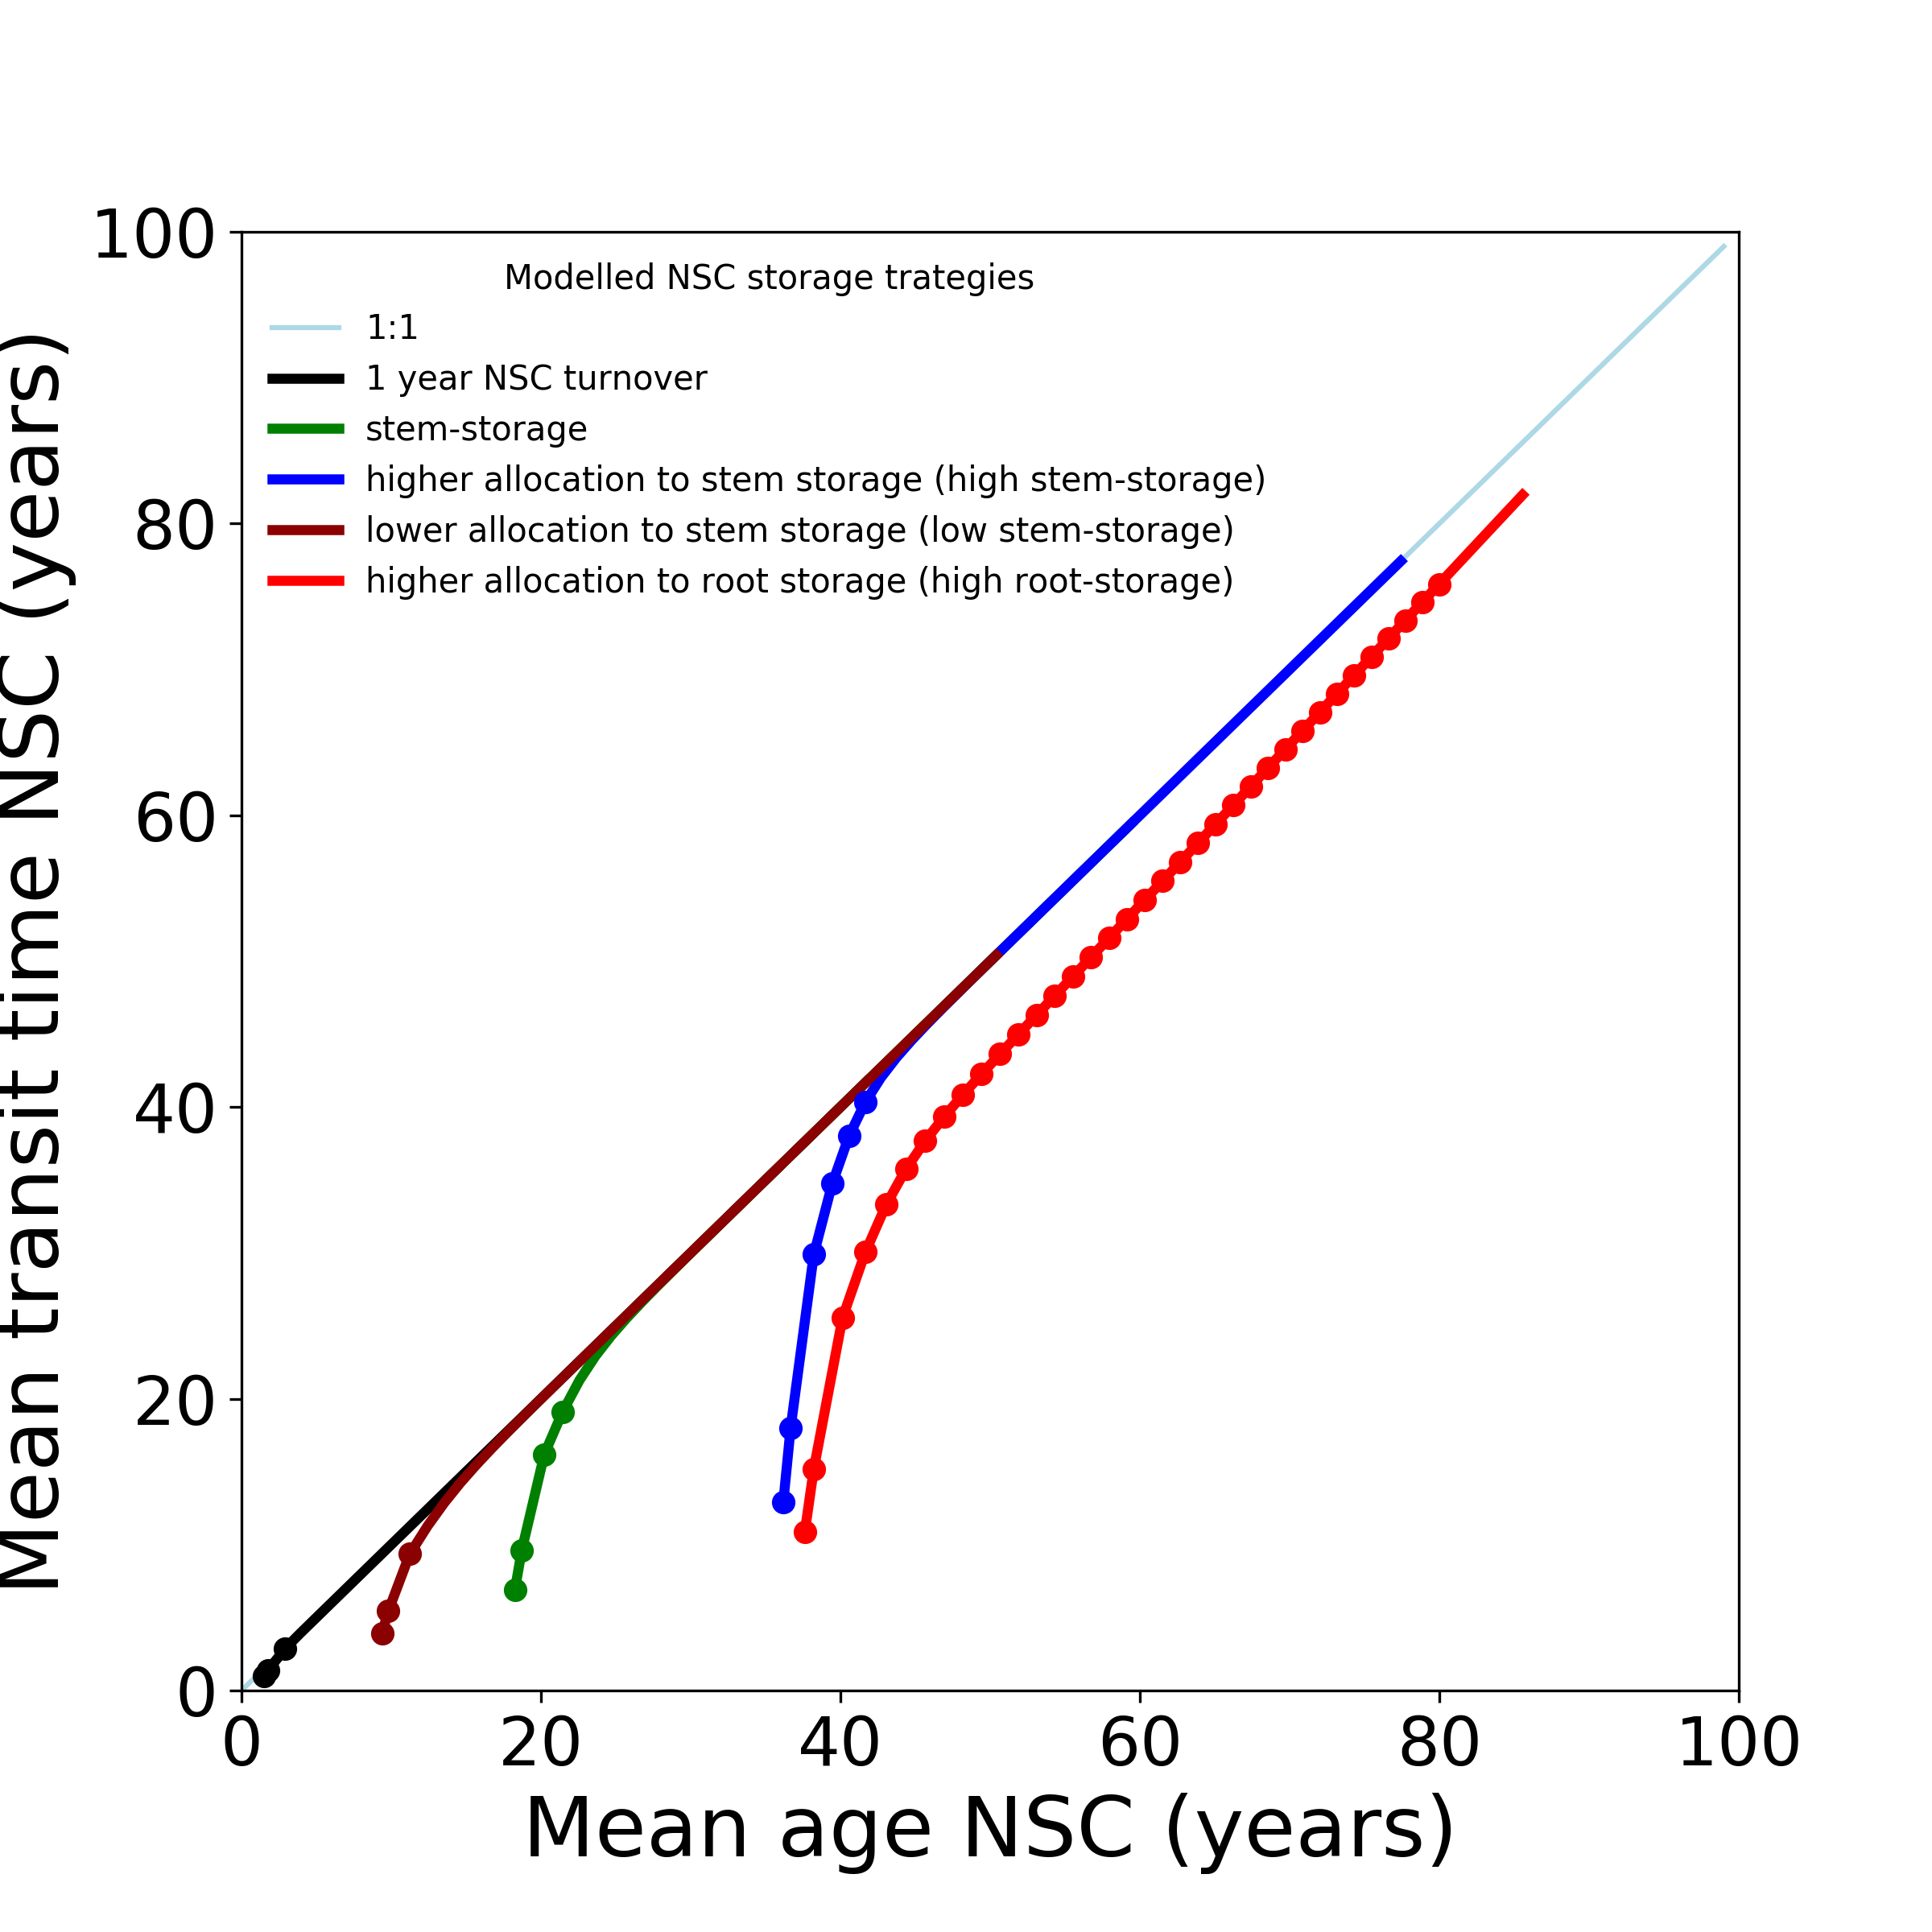
\includegraphics[width=5in]{Starvation_different_trees.png} 
   \caption{Simulation of the pathway that the metabolic safety margin wold follow when trees face starvation for each of the simulated trees specified in the Table\ref{table:parameters}. Each poin in each trend line represents one time step of one year. The amount of point each line has before reaching the 1:1 line shows te amount of years each of those trees would take to exahust their NSC reserves}
   \label{fig:starvation}
\end{figure}


We also modeled the transient changes in the metabolic safety margin when trees expirience a limitation in the carbon supply.
In these simulations, income was kept as in Table \ref{table:parameters} for the first 10 yeas and then it was reduced to 2300 gC/year for the next 40 years. 
Here we compare a fast cycling tree (black line) with a slower cyclilng tree (gree line) (Fig. \ref{fig:income_reduction}). 
A reduction of the carbon income produce a transient response in the metabolic safety margin for both trees (Fig. \ref{fig:income_reduction}). 
Metabolic safety margin approached the 1:1 line as trees get depleted of carbon, and then they come back to steady state while all the carbon gets replaced by new carbon under the new conditions (Fig. \ref{fig:income_reduction}).
In these new conditions the size of storage pools and carbon fluxes adapt to the new income keeping NSC turnover times constant. 
%At the end the relationship between mean age and mean transit time comes back to the initial steady state point, only NSC pool size and carbon fluxes get scaled.  
Depending on the NSC turnover some trees will take longer than others to come back to the steady state metabolic safety margin, the transient changes in the metabolic safety margin are faster in trees with faster turnover times (black line) than in trees with slower NSC turnover times (green line). 


If a tree expiriences increses in the NSC turnover times due to changes in environmental conditions, we would expect a shift in transient pathway of the metabolic safety marging from a slower (green line) to a faster (black line) response (Fig. \ref{fig:income_reduction}).
Then, when trees come back to steady state they would be closer to the 1:1 line as NSC turnover time increased.
These simulations help us understand the trajectories of the transient response of the metabolic safety margin to stress and perturbations, and help us to evaluate how changes in NSC turnover times would affect trees responses to stress.
This provide us a tool to evaluate trees' health and trees' potential ability to survive and recovery under stress and perturbations.  
%Nevertheless, this transient response of the metabolic safey margy would follow a similar patern, varying only in the times that the systems would come back to steady state. 
%For instance, if a slow cycling tree (green line in Fig. \ref{fig:income_reduction}) suffers a reduction of income, which reduces the stocks of NSC, but do not adjust the carbon fluxes to keep a constante turnover time, it will result in am increse in the NSC turnover time, probably accelerating the transient responses to stress and perturbations, resembling more the pathways observe for the black line in  Fig. \ref{fig:income_reduction}. 
%When NSC trurnover time changes as a consequence of the new coditions we wuld observe a change in the relationship between the NSC mean age and NSC mean transit time that would reflect a change of trees strategy of cycling carbon. 

 
\begin{figure}[h] %  figure placement: here, top, bottom, or page
   \centering
   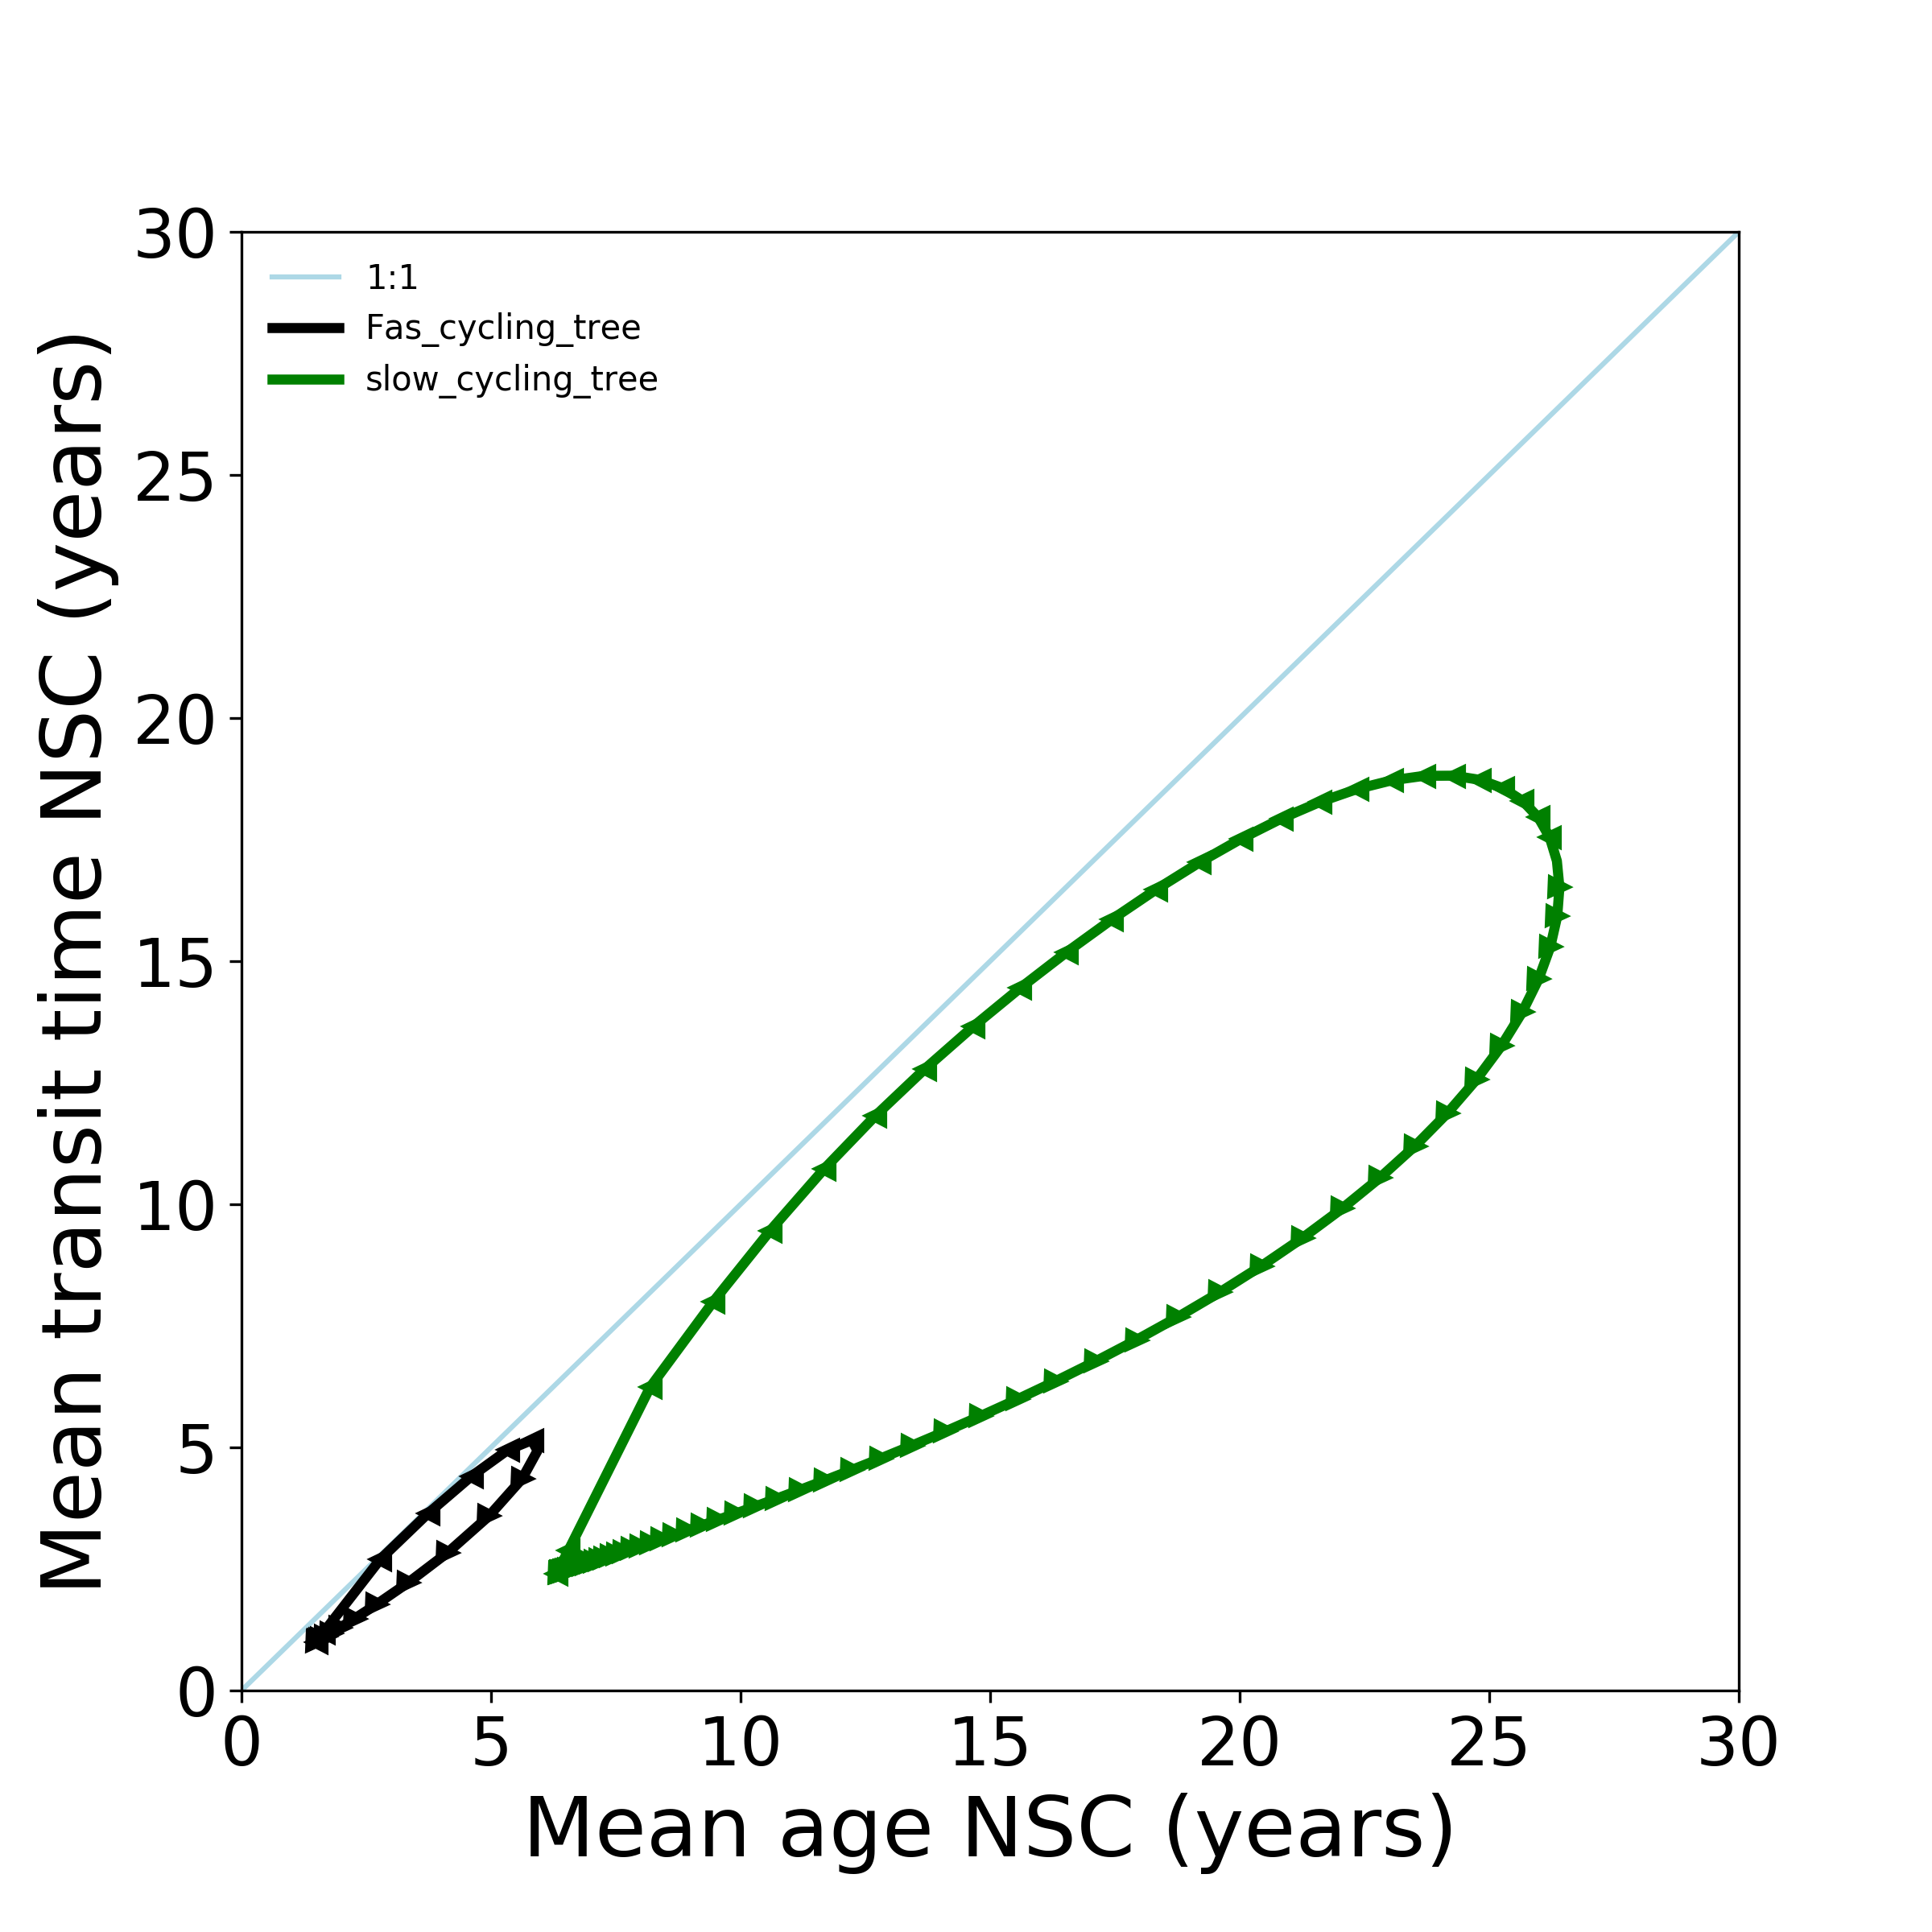
\includegraphics[width=5in]{income_reduction.png} 
   \caption{Simulation of the pathway that the metabolic safety margin of two trees with contrasting NSC turnover times would follow after facing a reduction in photosynthesis. The black line represents a tree with a fast turnover time, while the green line represents a tree with a slower turnover time. The arrows in the line show the direction of the changes at each time steps. Each arrow represent one time step (1 year)in the simulation.}
   \label{fig:income_reduction}
\end{figure}



%We run a simulation where we estimated the age and the transit time of the NSC. In the figure (\ref{fig:NCSage_simulation}) we show the estimated path that the relationship between the NSC age and NSC transit time would follow under a starving event in two trees with different storage status and metabolism. For instance, in Pinus halepensis we have very high reserves turnover time which leads to very young storage. For this species the relationship between NSC age and transit time gets closer to the 1:1 line very fast after a starving event. In A. rubrum, which have a slower NSC turnover time, reserves are older and when trees are not stressed transit time is very young. When these trees experience starving conditions the consumption of old reserves slowly takes the relationship between NSC age and transit time closer to the 1:1. 
%From these simulations we might estimate that this A. rubrum tree at year one would be more resilient to compounding disturbances than one P. halepensis tree at year one, but one tree of A.rubrum at year 7 would be equally vulnerable to disturbances that one P. halepensis tree at year 2. 
%
% \begin{figure}[h] %  figure placement: here, top, bottom, or page
%   \centering
%   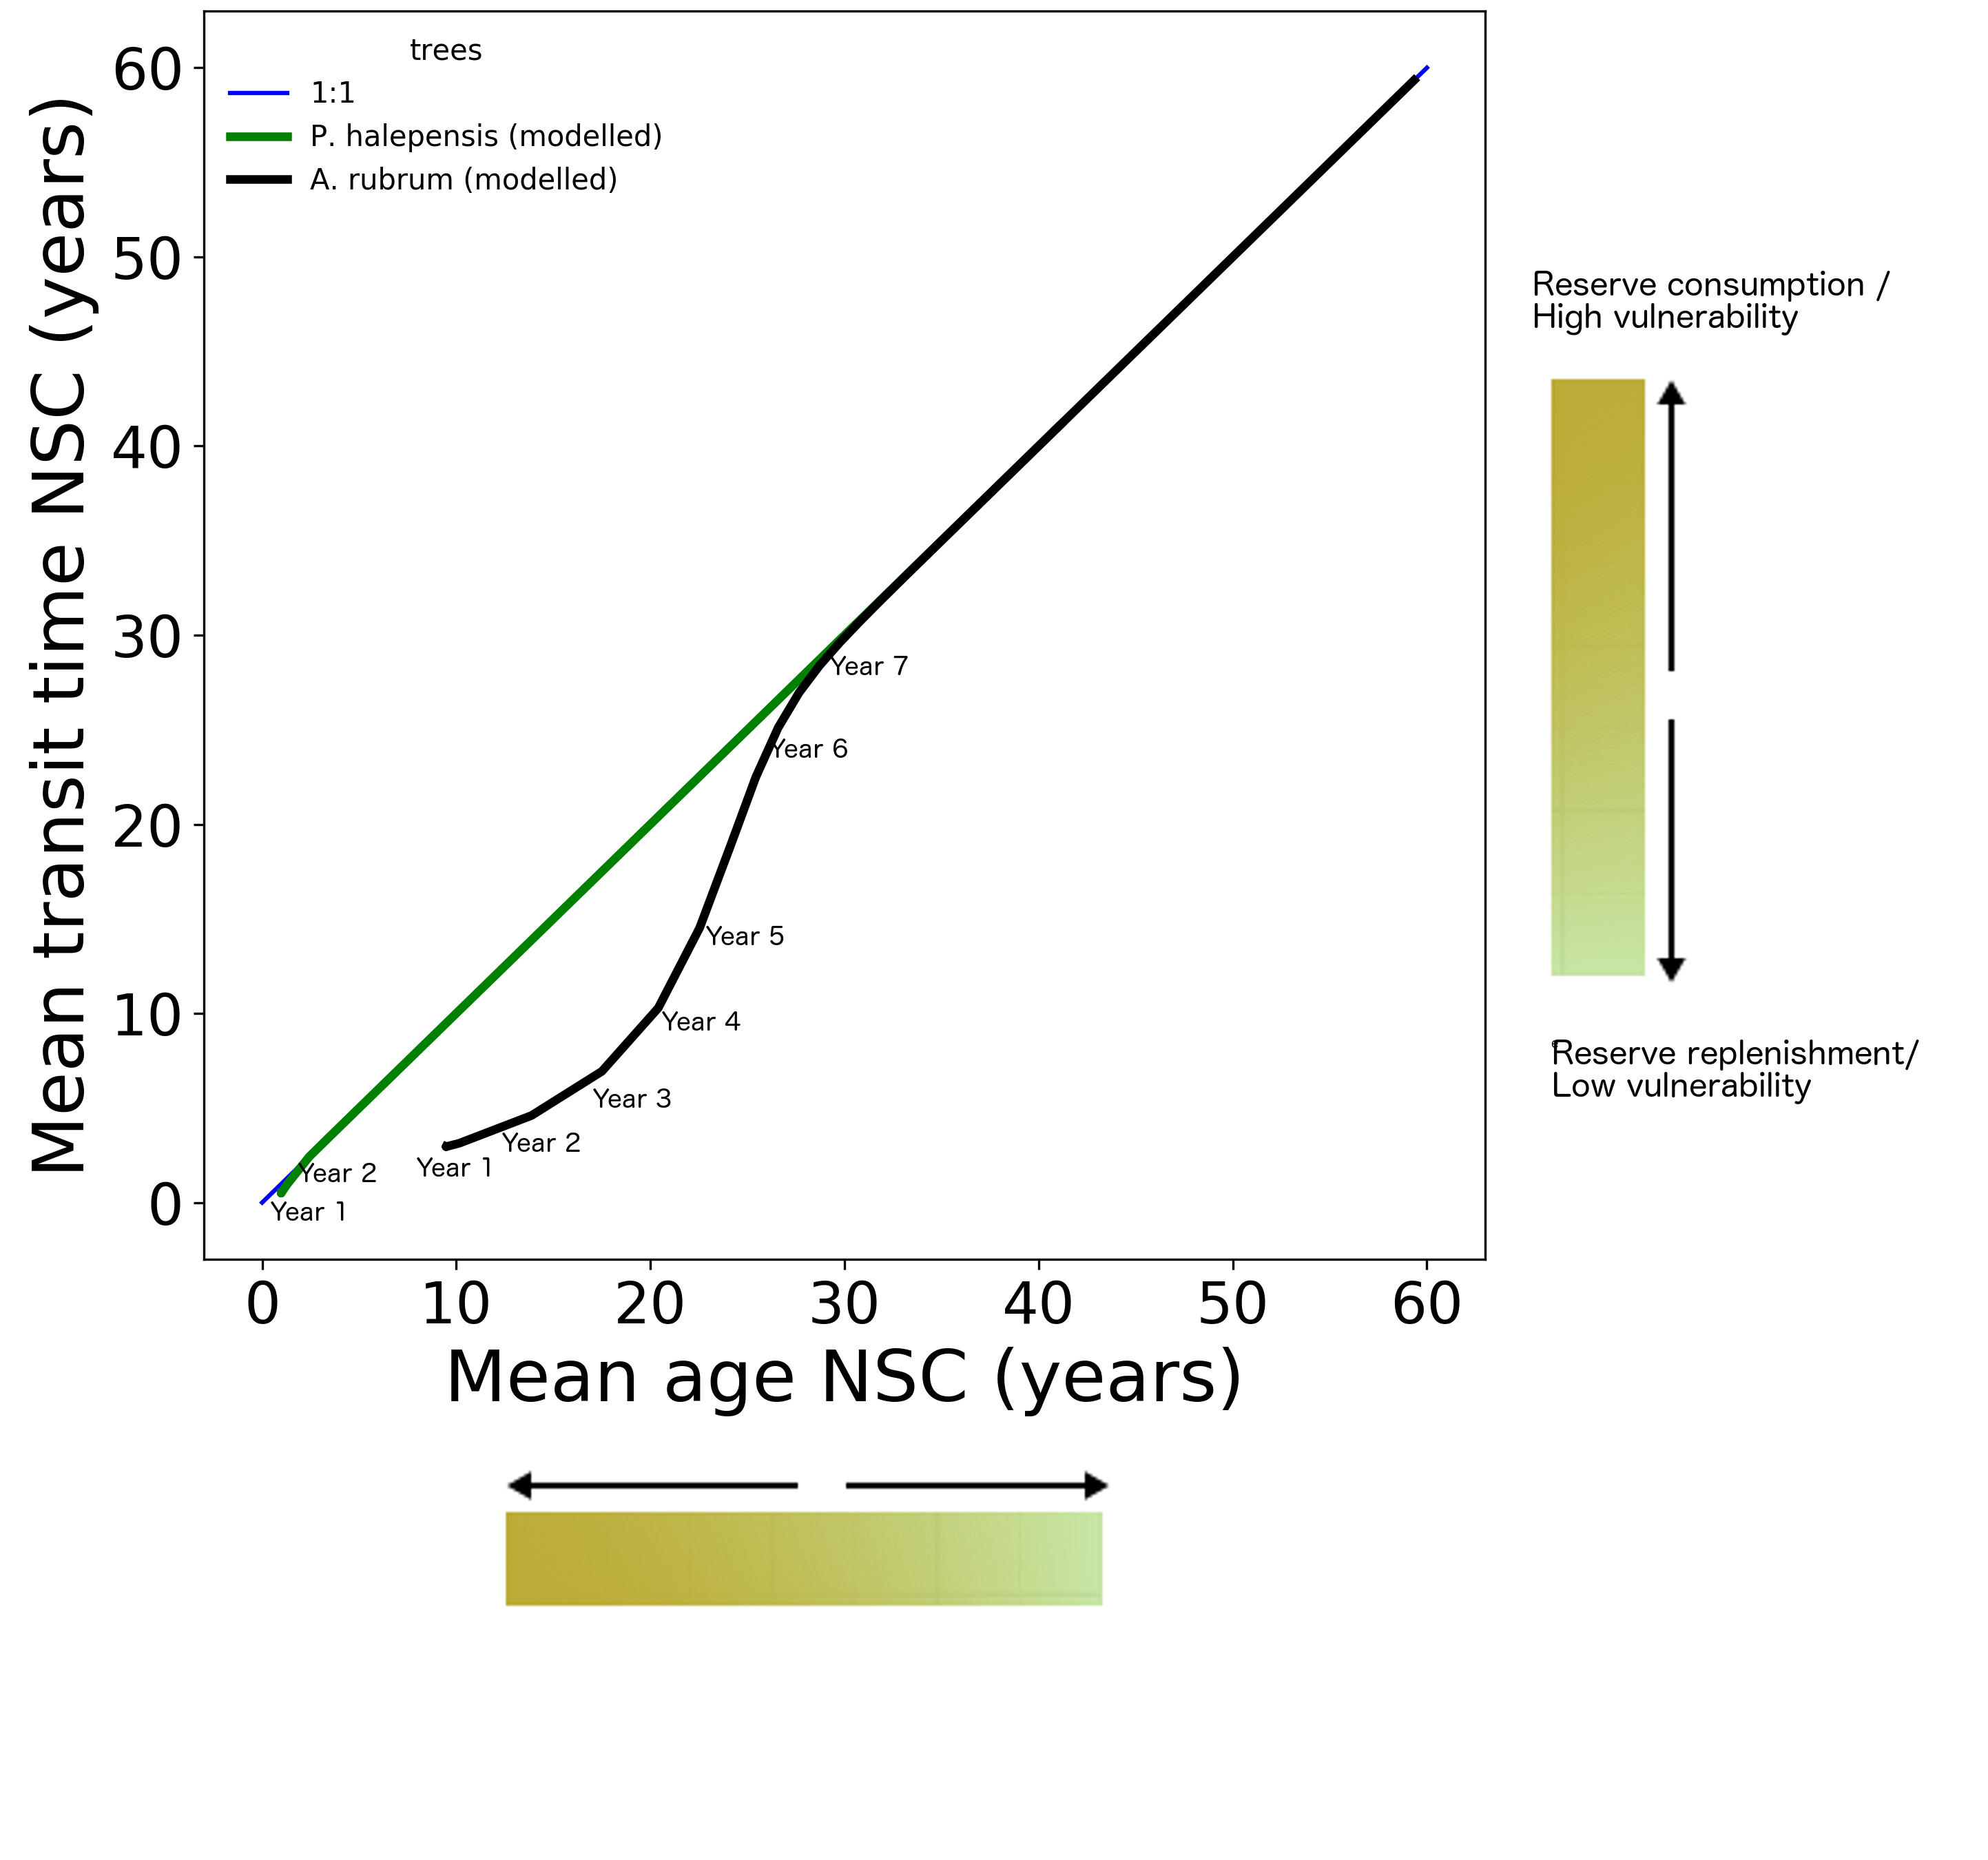
\includegraphics[width=5in]{starving_simulation.png} 
%   \caption{modelled trajectory of the relationship between NSC age and NSC transit time for two species with contrasting storage strategies (run this with different percentages of reduction).}
%   \label{fig:NCSage_simulation}
%\end{figure} 



%% We can also do a simulation where the income gets readuce by a proportion and track how the relationship gets older at the biggining of the simulation but bounce back to a recovery point after some time steps (probably to a point closer to the 1:1 line, showing a change in the vulnerability to starvation of the trees). Simulate a seay

\subsection {$^{14}C$ approach}

$^{14}C$ have been widely used to estimate the age of  NSC (soluble carbon and starch), the formation of new structural tissues (leaves, wood, roots) and the respired $CO_{2}$ in plants.
Using the bomb spike in the $^{14}C$ concentrations in the atmosphere, caused by the bomb testing in the 1950's and 1960's, $^{14}C$ measurements can be calibrated to calendar dates with only 1 year of uncertainty. 
%This technique provide us a good estimation of the mean age of the carbon in each tissue or organic compound measured in trees. 
Consiering only NSC in plants, we can assume that the age of the NSC could be estimated by the $^{14}C$ signal of the stored NSC (soluble sugars, starch and lipids), while the NSC transit time could be estimated with the $^{14}C$ signal of the carbon allocated to build new biomass (growth) and allocated to respiration ($CO_{2}$).

Estimates of the NSC ages based on $^{14}C$ gives an average value of the distribution of the NSC age in the analyzed sample. 
This may not represent well NSC age distribution as they may be skewed distributions towards younger values of NSC ages, and makes estimation of the NSC ages for the entire tree difficult.  
%This also difficults the estimate of NSC age distribution of different tree organs based on $^{14}C$ measurements. 
Nevertheless, to date, $^{14}C$ measurements are our best approach to characterize mean NSC ages and transit times in tree organs and compounds, and observe their changes when trees face stress or perturbations. 
It is important to identify what are the key organs and compartments where estimates of the metabolic safety margin would give us insights about the metabolic state of the whole tree, helping us to estimate the metabolic vulnerability of trees to upcoming stressful conditions. 

\subsubsection{What organs should we measure to estimate trees' metablic safety margins?}

 $^{14}C$ ages are not evenly distributed in trees, different tree organs have different age composition depending on trees species and organ dynamics. 
For instance, leaves will generally have very young NSC because they cycle it daily, while stemwood and coarse roots would have an age composition with larger proportions of older carbon because their NSC cycling would reflect multiannual dynamics. 
Then, if metabolic safety margins would inform us about how well prepare are trees for future uncertain conditions at multiannual scales, mean NSC ages and transit time of long term reserves such as the ones in stem wood and roots would give us a good estimate of the metabolic state of trees.  
Stem wood reserves can serve as an integrator of carbon dynamics in the whole tree. 
$^{14}C$ mean ages of NSC have been reported to be older in stem wood and coarse roots than in any other tree organ. 
These ages show a large variability depending on the tree species and environmental conditions. 
It has been shown that trees access these reserves to support metabolism during girdling experiments, where the $^{14}C$ age of the $CO_{2}$ comming from the stem wood became progressively older with time while trees use their stored NSC. 
Trees also used their carbon reserves to rebuild new tissues in order to recover after a cathastrophic event, where $^{14}C$ ages of the carbon use tu build new branches and roots resemble the ages in te NSC pools of the stem wood and coarse roots.
Therefore, measuring the $^{14}C$ in the NSC reserves and respired $CO_{2}$ in the stem wood would can be use to have a good proxy of the metabolic safety margin of the entire tree for mature trees. 
%Aditionally, The quantities of NSC that compound each carbon pool are different and difficult to estimate, then it is very challengin to estimate weighted averages for the $^{14}C$ measurements of the entire tree when the relative contribution of each pool is unkown. 

%The NSC pools int the stemwood and coarse roots cycle slower than other pools, and they supply carbon to the other faster pools during times where new carbohirates are limited.
%Then these pools would be more sensitive to changes in metabolic conditions that affect trees carbon dynamics than faster poools. 



%Then we believe that footprints of the entire tree carbon metabolism are recorded in the NSC mean age of the stored reserves in the stemwood and the mean age of the NSC being respired or allocated to growth in the stemwood. 



%These may  be the largest NSC pools that would support metabolism when trees face stress and need to recover from damage.
%Then measurements should focus in these two storage pools. 
%Althoug it may be difficult to average independent measurements of these two pools together, it would be informative to have both estiamtes.
%Alternatively, considering measuring only the low stemwood would give enough information to estimate the metabolic safety margin of mature trees. 
%stemwood is the largest long term storage pool, and it is the comon pathway of metabolically active NSC.


\subsubsection{What compounds should we measure?}

As stated before, NSC is mainly soluble sugars, starch and neutral lipids.
They all serve as storage reserves, but they may have different physiological funcionts as well. 
Soluble sugars would also be involved in osmoregulation, cell signalling and comunication, and can act as hormons, which are vital function for trees that need to be maintain. 
Neutral lipids may be involved in defense, stress responses, hormone signaling pathways, and celular transport, as well. 
Therefore, there may be a proportion of soluble sugars and neutral lipids that may not be accessible to support metabolism and growth in mature trees.

Starch seems to have the solely function of carbon and energy sotrage, which is accessible to support other metabolic and physiological functions. 
There are still uncertainties about the accesibility of all the starch reserves for supporting trees metabolism. 
Neverhteless, there is evidence that trees can remobilize almost completely all starch reserves in the leaves and in the stemwood, at different scales and in response to perturbations. 
This may indicate that most of the starch pools may be entirely accessible to support metabolism during stressful conditions or for recovering from perturbations. 


Estimating the ager of the starch using $^{14}C$ could be the best proxy of the mean age of the NSC to estimate the matabolic safety margins in mature trees. 
Starch dynamics may be a metabolic integrator of the trees carbon dynamics, and it can serve as a metabolic integrator of the whole tree metabolism. 
It is possible to isolate starch for $^{14}C$ using enzymatic extraction methods, paying special attention in avoiding contaminations with exogenous carbon. 
Alternatively, estimating the age of the soluble carbon using $^{14}C$ may be a viable alternative. 
Soluble carbon is esier to extract than starch, although it may not represent 100\% of the accessible reserves, if we assume a fast interchange beteween all soluble carbon (sugars, proteins, tanins, etc) and starch reserves in the sampled organ, the age of soluble carbon would also be a reliable representation of the NSC mean age. 
%When isolating soluble sugars, other soluble compounds such as proteins and tanins could be extracted and measured, and would add noise to the measurements. 
Here, we propose the use of $^{14}C$ measurements of starch as the best proxy for the NSC mean age of the storage compartments, but the use of soluble carbon may also give valuable information in case of lacking the thecnical capacity for starch isolation. 


To estimate the metabolic safety margin we still need to estimate the NSC transit time.
As stated before, NSC transit time is the carbon allocated to metabolism (mainly respiration and growth).  
I we assume that cell respiration is a priority over growth.
Then changes in the age composition of the emited $CO_{2}$ would be more sensitive to changes in the metabolic conditions of trees following stress or perturbations than the age composition of carbon alloated to growth.  
Therefore $^{14}C$ of te respired $CO_{2}$ wold be a good proxy of the transit time of the acccesible NSC stored in any tree organ.  
We haypothesize that, metabolic safety margin for mature trees would be more informative if the mean age of the NSC and mean transit times are estimate form the stored starch pools and the respired $CO_{2}$, respectively, in the stem wood or roots.

%There is evidence that show that growth is quickly stop when trees face stressful conditions or are photosythetically limited, while the maintainance respiration is maintained at minimal levels. 
%Generally wood growth is done with recently formed NSC with very little contribution from old stred NSC.


%\subsubsection{When to measure?}
%
%NSC is higly dynamic over time, reflecting the tranient balance between carbon sources and sinks.
%Then the $^{14}C$ of the NSC and the respired $CO_{2}$ would slightly change depending on the short term metabolic state of the NSC.
%If trees are experiencing a transient seasonal stress like the dry season values would tend to be older than when trees are experiencing a transient positive carbon balance during the wet season. 
%if conditions of stress are regular, and we want to know the long term metabolic safety margin of the tree, chances are higher to have a better signal if measurements are taken during the dry season, or during the expected peak of stress. 
%Nevertheless it would be very informative to capture the seasonal fluctuation of the metabolic safety margin, and this informatio would help us understand how trees respond to periodic strees.   

\subsubsection{Some examples}

We estimated the metabolic safety margin measured at different organs to test our hypotheses in different sets of trees.

We did these measurements on tropical trees growing at a seasonal dry forest in Mato grosso, Brasil. 
We measured species with contrasting storage traits (starch storage in the parenchyma cells and starch storage in the living fibers) to evaluate if differences in the prioritization to storage can be detected in the metabolic safety margins.
We also measured during the wet and the dry season to evaluate the impact of seasonal stressful conditions on the metabolic safety margin. 
Additionally, we measured these quantities in the branches and roots of \textit{Larix decidua} and \textit{Pinus mugo} growing in the Swiss Alps to evaluate the representatitvity of the storage organ in the metabolic safety margin. 
 
Estimates of the NSC mean age were done based on  $^{14}C$ measurements of soluble carbon extracts from stem wood cores following the methods described in Hillman et al...
Estimates of the $CO_{2}$ ages were done based on  $^{14}C$ mesurements of the $CO_{2}$ incubted from stem wood cores following the methods described in mhur et al, hilman et al and pltier et al. 
The incubations were done for 36 hours to estimate the age of the cabon allocated to respiration at the moment of sample collection, avoiding remobilization of older, long-term, reserves. 

Our measuremens show that there are differences in the metabolic safety margin measured in the stem wood beteween storage strategies for the tropical trees in the Amazon (Fig. \ref{fig:14C_measurements}).
Fiber storing species, which prioritize allocation to NSC, have lower metabolic safety margins than parenchyma storing species (Fig. \ref{fig:14C_measurements}), where most of the trees are far away from the 1:1 line in Figure \ref{fig:14C_measurements}. 
Seasonality in precipitation also seems to have an effect on the metabolic safety margin, reflecting the impact of the dry season on trees metabolism and use of storage reserves. 
During the dry season (July 2018) the metabolic safety margin was closer to the 1:1 line for most o the measured trees, while during the end of the wet season (May 2019) all trees show a recovery of the carbon reserves reflected in younger mean ages and younger mean transit times (Fig. \ref{fig:14C_measurements}).

We observed differences in the metabolic safety margins estimated from different tree organs.
In our measurements in \textit{L. decidua} and \textit{P. mugo}, branches show younger mean ages and transit times than 1-2mm roots (Fig. \ref{fig:14C_measurements_sweeden}), indicating an appearent higher turnover time in NSC in the branches than in the roots, which is in agreement with previous studies. 
Furthermore, differences in the metabolic safety margin between species can be observed only for root ramples (Fig. \ref{fig:14C_measurements_sweeden}), which store older reserves and may be better reflecting long term metabolic dynamics of trees. 
This supports our hypothesis that evaluating metabolic safety margins in roots and stem-wood would give more information about the metabolic state of the tree than organs with faster turnover times. 


\subsubsection{Important technical considerations about sampling $CO_{2}$ to estimate NSC transit time}

Tissue specific incubations may be the most efficient whay to collect $CO_{2}$ to estimate NSC transit time for the tissues of interest. 
When sampling for the stemwood or roots, some considerations should be taken: 

\begin{enumerate}

\item   Respiration should be obtained only from the living wood core, phloem and heartwood should be excluded.
Sometimes when it is difficult to determine where the sapwood ends, it would be useful to use lugol iodine in the wood core to identify the proportion of living wood to be incubated. 
Incubating heartwood may influence the $^{14}C$ measurementes because it would also reflect the respiration of other microorganism that are feeding from the structural carbon in the heartwood. 
Descomposition of heartwood can generate not only $CO_{2}$ coming from the microorganisms in the wood but it would also collect methane $CH_{4}$ that would contaminate $^{14}C$ measurements of the collected material and would alter the estimations of NSC transit time. 

In the same sense, incubated sapwod should not be extremely infected by fungi or bacteria.
If the level of infection is high then the collected $CO_{2}$ may maily reflect the respiration of microorganism and not wood respiration. 


\item  $CO_{2}$ easily disolves in the sap and it is transported vertically in trees. Incubation of woody tissues inmediatelly after collection would collect $CO_{2}$ that has not been respired directly by the incubated tissue, but $CO_{2}$ that was respired somewhere else and transported in the sap. 
After collecting the woody tissue, it should be left to estabilize with the ambient air for around 1 hour before incubation starts, in order to avoid contamination from transported $CO_{2}$. 

\item  Wood or roots are living tissues that after collection would eventually start dying. 
There is a lot of uncertainty when living cells in the wood or roots would start dying after being excised from the tree, and what would caused their mortality. 
Nevertheless, we believe that extreme heat and dryness will contribute to accelerate dying of wood and root cells once collected. 
We recomend that after collection, tissues should be kept humid and in a fresh place to avoid premature death. 


\item  For incubtions to reflect the transit time of the NSC in the stem wood or roots, they should not last long, the shorter the better, in order to avoid remobilization of the wood core storage reserves that would not be accessed if the wood core would have remained in the tree. 
Incubating tissues for many hours would results in the collection of the $CO_{2}$ corresponding to all the available reserves, as long as the wood tissue remains alive and respiration from growing fungi and bacteria remains negligible. 
The goal is to collect enough $CO_{2}$ to measure $^{14}C$ in the shortest time possible, and this would depend on the respiration rates and the quantity of the incubated living tissue. 
Neverhtless, we recomend incubation not to last more than 48 hours. 
This threshold would avoid remobilization of storage reserves that were not being used by trees at the moment of sampling, and the infulence of microorganisms that would start growing in the tissue after a couple of days of the incubation.  

\end{enumerate}

%Transit time is the age of the carbon that is leving the NSC system at the moment of sampling. 
%when sampling wood cores, and they stay salive for several days, incubations would become a starving situation when they have to start tapping on the reserves to respire. 
%Incubations should be restricted to the first hours of respiration after collection, before wood cores strat remobilizing long term stoage. 
%Evidence suggest that $^{14}C$ wont radically change after 48 hours of incubation. 
%We would recomend keeping this limit to avoid complications with the $^{14}C$ measurements. 
%
%Alternatives to wood core incubation can be stem incubations. 
%chambers with flasks can be installed directly in the stem of the trees and $CO_{2}$ can be collected from the direct respiration of the stem. 
%this $CO_{2}$ would represent several respiration sources that should be accounted for: 1) they integrate respiration from wood, phloem and microorganismos living in the bark; 2) it may also collect $CO_{2}$ bein axially transported in the sap; and 3) it could also collect methane being transported throug the stem from the soil, or bein produced by heart wood decomposition or by insect invasion. 

    


%
%$^{14}C$ measurements can help us estimate the mean age of the stored NSC and its transit time. 
%
%The stored NSC is compound of soluble sugars, starch and lipids. Nevertheless, starch is the only compound that seems to have only the function of storage. alternatively, it is easier to isolate for $^{14}C$ measurements without risk of contaminating it with other sources of carbon. Therefore, a good approximation to the mean age of the NSC would be the $^{14}C$ age of the the stored starch in the stem wood and woody roots.
%
%NSC Transit time is the time a particle of NSC would leave the system. When considering only the NSC system in a tree, this carbon can leave the system when it is allocated to respiration, growth, defence compounds, exudates and reproduction. Here we might assume that trees would prioritise to keep the minimal level of respiration under stressful conditions and therefore estimating the $^{14}C$ age of the respired $CO_{2}$ would be an adequate approximation to estimate the mean transit time of the NSC in a given tree organ. 
%
%Measurements of these quantities in living trees would allow us to distinguish how far away are these trees from the 1:1 line and therefore estimate their vulnerability to compounding disturbances, and the affectation of some disturbances to their carbon metabolism such as a strong dry period. in the figure  (\ref{fig:14C_measurements}) we show some measurements done in three tropical species. Here we can tell that some trees are very close to the 1:1 line and also have very young storage which would make them very vulnerable to many stressors. 
%Some other individuals have built a very old storage as they use younger and recently fixed carbon for respiration, these trees may have better possibilities to stand disturbances and recover from them. 

%% here we can include info abour the mean ages of those trees, where the oldest trees are the ones more distant to the 1:1 line, and therefore they may. haver survived and recovered from many disturbances. We can also argue about the differences in the species, species with shorter life span likde O. leu and S. gui have individuals on average closer to the 1:1 than individuals from D. mic. 

 \begin{figure}[h] %  figure placement: here, top, bottom, or page
   \centering
   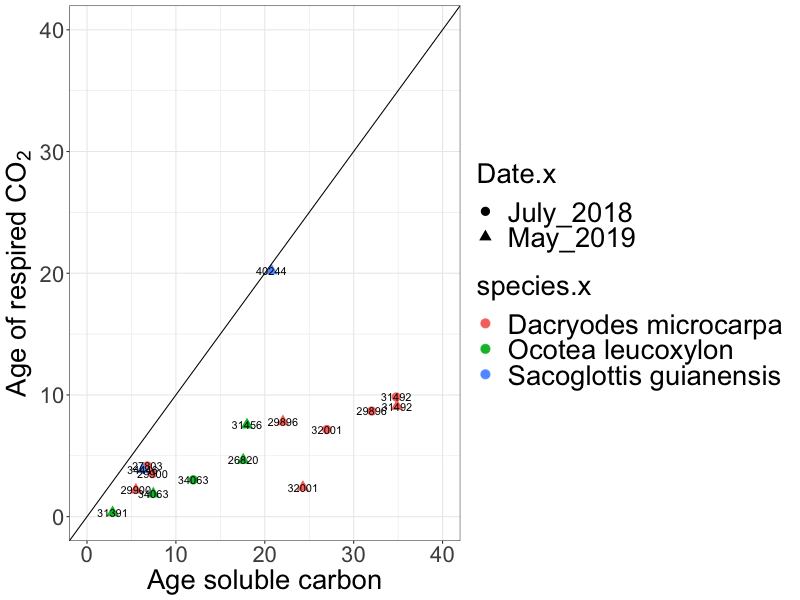
\includegraphics[width=5in]{Tanguro_trees_wet_dry_season.png} 
   \caption{Estimates of the matebolic safety margin for trees measured in a seasonal dry forest in the Amazon during the wet and the dry season. We estimate the age of the soluble carbon and the respired $CO_{2}$ using $^{14}C$ measurements and the bomb spile callibration curve.}
   \label{fig:14C_measurements}
\end{figure}

\begin{figure}[h] %  figure placement: here, top, bottom, or page
   \centering
   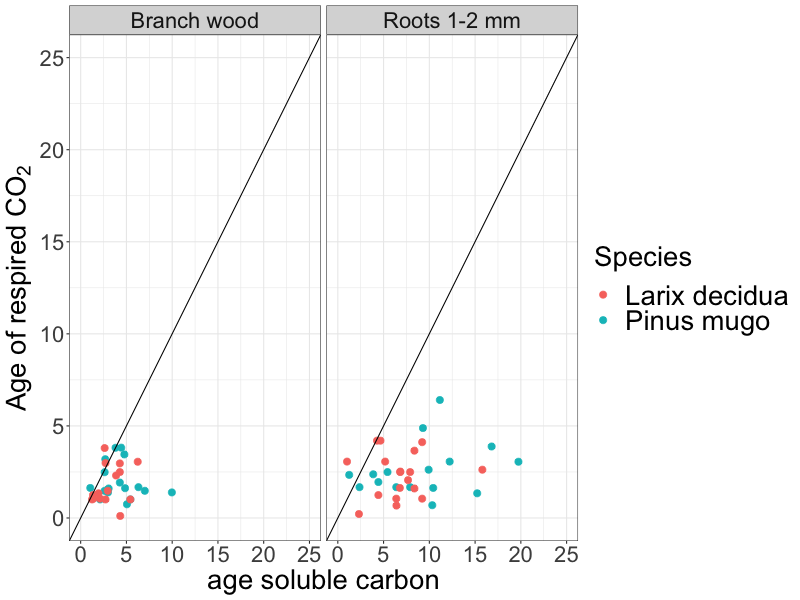
\includegraphics[width=5in]{Sweeden_trees_branch_fineroots.png} 
   \caption{Estimates of the matebolic safety margin for \textit{Larix decidua} and \textit{Pinus mugo} in the swiss alps. We measured branches and roots from the same individuals. We estimate the age of the soluble carbon and the respired $CO_{2}$ using $^{14}C$ measurements and the bomb spile callibration curve.}
   \label{fig:14C_measurements_sweeden}
\end{figure}

%\subsection {estimates of the NSC mean age and transit time based on pulse 13C or 14C pulse label experiments}
%
%This experiments with a intensive measurement of the depletion of the label could give us the entire transit time and age distribution of the carbon in the NSC tree system. 
%

\subsection{Utility of the new hypotheis}

Here we presented a new theoretic framework to evaluate the metabolic vulnerability of trees to future frequent and severe stress or perturbations. 
this framework help us evaluate and undertand the metabolic status of mature trees at a given time point, integrating the life history traits and storage dynamics of trees. 
From this metacolic state it can be estimated the potential turnover times of the accessible NSC reserves which influence the time that trees can rely on those reserves to survive and recover from stress or perturbations. 

This theory also has the potential to help us undertand patterns of recovery and adaptation in adult trees. 
Evaluating how NSC turnover times change in trees in response to stress and perturbation, measuring changes in the the matebolic safety marging, will help us undertand how NSC dynamics are affected by changes in environmental conditions and to assess the capacity of trees to recover from those changes. 
Informatin regarding the accessibility of NSC reserves and changes in NSC turnover times in response to environmental changes is still scarce. 
Our propose framework offers a viable alternative to evaluate how appearnt  NSC turnover times would change when trees are expose to evironmental changes or have to face multiple perturbations.  

%
%Our hypothesis would open a new ways to evaluate trees and forest health and its capacity to recover from environmental changes. 
%there are still a lot of uncertainties about how trees survive and recover from perturbations and stress. 
%We are ineficient in the way to predict what determines if a tree would sorvive and recover from perturbations and stress. 
%Existing signals require time series and multiple measurements over time, which are challenging, costly and time consuming. 
%Furthermore, we have focuse a lot on understanding water dynamics and its contribution to forest and tree vulnerability and we have little focus on how carbon allocation and metabolism play  a significant role in forest resilience. 
%This new haypothesis allow us to study how different allocation strategies would impact the ability of trees to survive and recover and will give us tools to evaluate the metabolic vulnerability of trees to environmental changes. 

%\subsection{challenges and caviets}
%
%\begin{itemize}
%\item Parametrise pool models to run simulations is difficult and time consuming.
%\item Measuring only the 14C of starch and respired $CO_{2}$ may bias the estimation of the mean age and mean transit time for some tree species as other storage compounds may be more relevant than starch for some species and allocation of carbon to reproduction, exudates and defence compounds may be more relevant to the transti time estimation than the respiration?
%
%\item discuss the probabilities and conditions when either matematically or by estimation of meand ages and transit times based on isotopes the relationship between mean age and mean transit time is over the 1:1 line. Math processes and model structure! when for instance carbon enters to the system through one pool very in the beginning and then goes out several pools later.  
%
%\item analyze the caviets about the difficulties to explore all the 14C respired from different tree organs and the stored NSC in different tree organs. Also when focusing only on the storage tissues "because it is the oldest NSC in the system" what are the methodological challeneges. For instance, is respiration of old NSC in deep tissues increased by exposition of the wood too larger amount of oxigen? 


%\end{itemize}

%\subsection{Conclusions and future questions}
%
%are these characteristics philogenetic? 
%

\end{document}
